\documentclass[11pt,a4paper]{article}

% Essential Packages
\usepackage[utf8]{inputenc}
\usepackage[T1]{fontenc}
\usepackage[english]{babel}
\usepackage{graphicx}
\usepackage{float}
\usepackage{geometry}
\usepackage{amsmath}
\usepackage{amssymb}
\usepackage{rotating}
\usepackage{booktabs}
\usepackage{multirow}
\usepackage{microtype}
\usepackage{siunitx}
\usepackage[authoryear,round]{natbib}
\usepackage{parskip}
\usepackage{setspace}
\usepackage{tabularx}
\usepackage{lineno}
\onehalfspacing

\IfFileExists{newtxtext.sty}{\usepackage{newtxtext, newtxmath}}{\usepackage{mathptmx}}
\usepackage[font=small, labelfont=bf, margin=1cm]{caption}
\usepackage{authblk}
\usepackage{xurl}
\usepackage{xr-hyper}
\usepackage[colorlinks=true, allcolors=blue]{hyperref}
\usepackage{cleveref}
\externaldocument[M-]{main}
\usepackage{tikz}
\emergencystretch=2em
\usepackage{quantikz}
\usetikzlibrary{shapes.geometric, arrows, positioning, fit, backgrounds}

\usepackage{xcolor}

% TODO toggle: \showtodotrue shows the notes, \showtodofalse hides them (submission version)
\newif\ifshowtodo
\showtodofalse
\makeatletter
\newcommand{\todo}{\@ifnextchar\bgroup\@todowitharg\@todonoarg}
\newcommand{\@todowitharg}[1]{\ifshowtodo{\textcolor{red}{\textbf{[TODO: #1]}}}\fi}
\newcommand{\@todonoarg}{\ifshowtodo{\textcolor{red}{\textbf{[TODO]}}}\fi}
\makeatother

% Fail compilation if a figure is missing (prevent silent placeholder boxes)
\graphicspath{{figs/}{./}}
\newcommand{\safefig}[2]{\IfFileExists{#1}{\includegraphics[width=#2]{#1}}{\IfFileExists{figs/#1}{\includegraphics[width=#2]{figs/#1}}{\PackageError{safefig}{figure file \detokenize{#1} not found. Run scripts/make_paper_figs.py first.}{}}}}

% Page Geometry
\geometry{top=2.5cm, bottom=2.5cm, left=2.5cm, right=2.5cm}

\title{\textbf{Supplementary Material to: Limits of Resolution in Quantum Machine Learning: A Statistical Noise Budget for Small Benchmarks}}

\author[1,*]{Enrique Real\,$^{\href{https://orcid.org/0009-0006-3862-9797}{\textnormal{\scriptsize [ORCID: 0009-0006-3862-9797]}}}$}
\affil[1]{Independent Researcher, Alicante, Spain}
\affil[*]{\textit{Corresponding author: enriquerb32@gmail.com}}
\renewcommand\Affilfont{\itshape\small}

\date{October 2026}

\begin{document}
\maketitle
\renewcommand{\thesection}{S\arabic{section}}
\setcounter{section}{0}
\renewcommand{\thetable}{S\arabic{table}}
\renewcommand{\thefigure}{S\arabic{figure}}
\renewcommand{\theequation}{S\arabic{equation}}

\section{Additional Methods}
\label{app:moved}

The map of experiments is \Cref{M-tab:expmap} of the main text.

\textbf{Experiment identifiers.} \emph{Core}: the matched train-only QML experiment of the main text (15 seeds, same 2{,}273 fitting rows, all probabilities stored; \Cref{tab:core_spec}). \emph{Rerun}: the train-only classical 15-seed reruns of Random Forest, XGBoost and the LSTM. \emph{Historical}: the canonical-pipeline experiments, whose per-seed AUCs were archived but whose per-seed test probabilities were not. For the four historical hybrids, the test probabilities of the seed-42 single run are stored, and seed-0 probabilities were regenerated afterwards; the regeneration reproduces the archived seed-0 AUC exactly for \texttt{LbL-QNN} and within 0.015 for \texttt{LSTM+QNN}, \texttt{LSTM+PI-QNN} and \texttt{LSTM+QTL} (\path{results_hybrid_perseed_probs.json}). The 15-seed train-only probabilities of all four variational hybrids belong to the Core experiment, which re-ran them on the dataset of the Rerun (\Cref{tab:core_spec}); no paired comparisons are made with the historical canonical-pipeline runs, for which only seed-0 probabilities exist. Historical results are descriptive and are not used for the inferential claims of the main text.


\subsection{Single-Seed Pairings}
\label{app:single_seed}
The main text compares the means of 15 seeds. For single runs, the paired standard error of two individual models is larger, and the verdict depends on which seeds are drawn.

\begin{table}[htbp]
\centering
\caption{Single-seed pairings: observed 15-seed mean gaps and minimum detectable differences (MDE $=2.80\times$ SE of the gap; $\alpha=0.05$, power 0.80). Standard errors are averages over the $15\times 15$ single-seed pairings; \Cref{M-tab:paired_ci} gives the comparison of the 15-seed means. MDEs are computed from unrounded standard errors, so they can differ in the third decimal from $2.80\times$ the SE shown. Last column: share of $15\times 15$ single-seed pairings declared significant.}
\label{tab:mde}
{\small
\resizebox{\textwidth}{!}{%
\begin{tabular}{lcccc}
\toprule
\textbf{Pair} & \textbf{Observed gap} & \textbf{SE of gap, iid / block} & \textbf{MDE, iid / block} & \textbf{Declared significant, iid / block} \\
\midrule
RF $-$ XGBoost & $+0.021$ & 0.013 / 0.014 & \textbf{0.036 / 0.039} & 27\,\% / 21\,\% \\
RF $-$ LSTM & $+0.015$ & 0.014 / 0.010 & \textbf{0.038 / 0.027} & 3\,\% / 24\,\% \\
XGBoost $-$ LSTM & $-0.007$ & 0.018 / 0.018 & \textbf{0.052 / 0.051} & 0\,\% / 0\,\% \\
\bottomrule
\end{tabular}%
}%
}
\end{table}

\textbf{Same-architecture control and single-seed detection.} Seed pairs of one model (e.g.\ seed $i$ against seed $j$ of Random Forest) are compared with the same two tests; the fraction declared significant is 1--4\,\% (DeLong) and 3--8\,\% (block). The classical models therefore rarely produce a nominally significant difference from seeds alone. The same check on the 105 seed pairs of each model of the train-only core experiment (\path{exp22_same_arch_core.py}) gives 2--21\,\% for the four variational hybrids (block 6--26\,\%; \texttt{LSTM+QNN} 2\,\%, \texttt{LbL-QNN} 11\,\%, \texttt{LSTM+QTL} 13\,\%, \texttt{LSTM+PI-QNN} 21\,\%) and 20\,\% for the Linear-4D control (block 22\,\%): for the models with the largest seed variance, a single pair of runs of the same procedure is declared significantly different in up to a fifth of cases. For cross-architecture pairs, all $15\times15$ combinations of seeds are compared.

\textbf{Historical contrast.} In the canonical runs RF $>$ XGBoost was declared significant in 66\,\% of the $15\times15$ seed pairings, RF $>$ LSTM in 7\,\% and XGBoost versus LSTM in 0\,\%, against 27\,\%, 3\,\% and 0\,\% in the train-only pipeline. The two sets of runs differ in the anomaly standardization and, for the tree ensembles, in the fitting rows (2{,}787 instead of 2{,}273); each model's 15-seed mean AUC moves by less than 0.005 between them, and with the rows held fixed the standardization alone moves the tree ensembles by at most 0.003 (\Cref{app:leakage_correction}). The canonical single-run gap RF $-$ LSTM was $+0.035$ (year-block bootstrap $p=0.001$; \Cref{sec:calibration_and_block_bootstrap}), against a train-only seed-mean gap of $+0.015$; because the preprocessing, the fitting rows of Random Forest and the training realization all differ, this contrast does not isolate initialization effects.


\subsection{Positive Control: Design}
\label{sec:positive_control_method}

The MDE is an analytical calculation; a positive control tests whether the benchmark behaves as predicted under controlled perturbation. Random Forest test probabilities $p_i$ are transformed to $\sigma(\text{logit}(p_i)+\varepsilon_i)$ with Gaussian noise $\varepsilon_i$, calibrating the noise scale so that the test AUC falls by a specified amount $\delta\in\{0.01,\dots,0.05\}$, with 15 seeds $\times$ 20 noise draws per $\delta$ ($\delta=0$ is a null control in which every detection is a false positive). We then count how often the benchmark declares the undegraded model significantly better (at $\alpha=0.05$). Two designs are used: the \emph{same-seed} design, in which the degraded probabilities are compared directly with the originating run (the loss $\delta$ is imposed exactly on the test set), and the \emph{different-seed} design, which is the realistic one because the compared models come from different training runs. Both are conditional perturbation experiments on the observed test set, not simulations from a known population: they check the detection machinery under one perturbation mechanism and do not establish coverage or power over new samples.


\subsection{Positive Control: Results}
\label{sec:positive_control}

\Cref{tab:positive} and \Cref{fig:positive_control} show how often the benchmark detects a Random Forest degraded by a known AUC loss. The 80\,\% detection point is reached at $\delta\approx 0.039$--$0.043$, consistent with the analytic MDE of the RF--XGBoost comparison. An imposed difference of 0.02 AUC, about the RF--XGBoost gap, is detected in only 17--30\,\% of runs. At $\delta=0$ the false-detection rate is 2--5\,\%, and for $\delta\ge 0.01$ no significant result had the wrong sign.

\begin{table}[htbp]
\centering
\caption{Positive control: percentage of runs in which the benchmark detects the undegraded Random Forest as better, as a function of the imposed AUC reduction $\delta$ (15 seeds $\times$ 20 noise draws per $\delta$). Entries are iid (DeLong) / block bootstrap. At $\delta=0$ every detection is a false positive.}
\label{tab:positive}
{\small
\begin{tabular}{lcccccc}
\toprule
\textbf{$\delta$ (imposed AUC reduction)} & \textbf{0.00} & \textbf{0.01} & \textbf{0.02} & \textbf{0.03} & \textbf{0.04} & \textbf{0.05} \\
\midrule
Same seed & --- & 8 / 15 & 20 / 30 & 52 / 62 & 84 / 80 & 97 / 92 \\
Different seeds & 2 / 5 & 7 / 12 & 17 / 27 & 47 / 57 & 75 / 76 & 93 / 92 \\
\bottomrule
\end{tabular}%
}
\end{table}

\begin{figure}[htbp]
    \centering
    \safefig{figs/fig_positive_control.pdf}{0.7\textwidth}
    \caption{Detection rate of a known AUC loss imposed on Random Forest. Dashed lines: same-seed design; solid lines: different seeds (the realistic design). The detection rate reaches 80\,\% at $\delta\approx 0.04$.}
    \label{fig:positive_control}
\end{figure}

The same-seed design fixes $\delta$ exactly on the test set; the different-seed design is the realistic one and is slightly less powerful below $\delta=0.04$.




\subsection{Specification of the QML Core Experiment}
\label{sec:core_spec}
\begin{table}[htbp]
\centering
\caption{Specification of the matched 15-seed QML core experiment (script \protect\path{exp17_hybrids_multiseed.py} with \texttt{-{}-fix-et0 -{}-p60 28.1}; outputs \protect\path{results_hybrids_trainonly_fixet0_p60_28.1.json} and \protect\path{results_hybrids_trainonly_fixet0_p60_28.1_probs.npz}, storing 528 test probabilities for every seed and model). The Random Forest, standalone LSTM, Linear-4D and \texttt{LSTM+QNN} classes and training loop are those of \protect\path{qml_core_trainonly.py}; the other three hybrids use the training code of the historical runs unchanged.}
\label{tab:core_spec}
\small
\begin{tabular}{@{}p{0.2\textwidth}p{0.74\textwidth}@{}}
\toprule
\textbf{Item} & \textbf{Specification} \\
\midrule
Pipeline & Train-only: anomalies standardized with years up to 1996 only; threshold $P_{60}=28.1$\,mm from the training partition; 35 input features. Identical to the dataset of the classical train-only rerun (the Random Forest and LSTM test probabilities agree with the rerun to within $10^{-11}$). An earlier execution of this experiment (\protect\path{qml_core_trainonly.py}) used a build in which \texttt{et0\_verano\_prev} and \texttt{potencial\_convectivo} were misaligned across stations and $P_{60}$ was 28.00\,mm; it is not used. \\
Rows & Fit: 2{,}273 training windows (1938--1996); validation: 514 windows (1997--2007), used only for early stopping; test: 528 windows (2008--2026). \\
Seeds & 0--14 for every stochastic model (\texttt{torch.manual\_seed} and \texttt{numpy.random.seed}; \texttt{random\_state} for Random Forest). The seed index is nominal across frameworks. \\
Random Forest & 300 trees, maximum depth 8, balanced class weights, mean imputation fitted on the 2{,}273 rows. \\
Standalone LSTM & 2-layer bidirectional LSTM (16 units per direction, dropout 0.3) over the first 12 input columns; its final states are concatenated with all input features, batch normalization, a 16-unit GELU layer (dropout 0.2, layer normalization) and a linear output. \\
Linear-4D control & 2-layer bidirectional LSTM (8 units per direction, dropout 0.2) over the first 12 input columns; projection of the LSTM states and features to 4 dimensions (dropout 0.1), sigmoid scaled to $[0,\pi]$, linear $4\to4$ map (20 parameters), layer normalization, linear output. \\
LSTM+QNN & Same as the control with the linear map replaced by a 4-qubit circuit (two repetitions of RY/RZ encoding followed by a strongly entangling layer; Pauli-$Z$ expectations; 24 trainable quantum parameters; \texttt{default.qubit}, backpropagation). \\
Parameter counts & \texttt{LSTM+QNN}: 2{,}368 (LSTM) + 208 (projection $51\to4$) + 8 (layer norm) + 5 (output) + 24 (circuit) = 2{,}613, of which 24 quantum (0.9\,\%); Linear-4D control: the same classical parts with the 20-parameter linear map instead of the circuit = 2{,}609. \\
Further hybrids & \texttt{LSTM+PI-QNN}: \texttt{LSTM+QNN} architecture trained with the heuristic thermodynamic loss (\Cref{app:heuristic_regularization}). \texttt{LbL-QNN}: 3-layer circuit trained layer by layer (10 epochs per layer) and then fine-tuned. \texttt{LSTM+QTL}: in each seed, a standalone LSTM is trained as above (its test probabilities are stored as the extractor) and frozen, and a quantum head is trained on it; the frozen extractor stays in training mode during this phase, so its batch-normalization statistics are updated and its dropout is active, as in the historical code. Hyperparameters in \Cref{tab:hyperparams}. \\
Neural training & AdamW (learning rate $5\times10^{-3}$, weight decay $10^{-4}$), learning-rate reduction on plateau (patience 3, factor 0.5), binary cross-entropy with positive-class weight, batch size 16, at most 25 epochs, gradient clipping at 1.0, double precision. \\
Selection & Early stopping on validation loss (patience 6, minimum improvement $10^{-4}$); the checkpoint with the lowest validation loss is restored. \\
\bottomrule
\end{tabular}
\end{table}
Equal capacity or tuning effort across the models should not be assumed. The \emph{Neural training} and \emph{Selection} rows apply to the standalone LSTM, the Linear-4D control and \texttt{LSTM+QNN}.

\subsection{Simulation: All Scenarios}
\label{app:sim_all}
\begin{table}[htbp]
\centering
\caption{All simulation rows. Population difference (Monte Carlo SE of the reference), rejection rate of $\Delta=0$ (number of rejections in brackets; DeLong, block bootstrap), coverage of the population difference, mean of the estimates, SD of the estimates and mean standard errors (DeLong, block). Scenario B first run: the Monte Carlo standard error of the reference was not recorded. Scenario A values are those of the first script run, rounded.}
\label{tab:sim_all}
{\scriptsize
\resizebox{\textwidth}{!}{%
\begin{tabular}{lcccccccc}
\toprule
$\Delta_{\text{true}}$ & \textbf{Rej. DeLong} & \textbf{Rej. block} & \textbf{Cov. DeLong} & \textbf{Cov. block} & \textbf{Mean $\hat\Delta$} & \textbf{SD$(\hat\Delta)$} & \textbf{SE DeLong} & \textbf{SE block} \\
\midrule
\multicolumn{9}{l}{\emph{Scenario B: shared year effects ($\tau_\pi=\tau_s=0.3$)}} \\
0.0000 (0.0002) & 0.040 (20) & 0.074 (37) & 0.960 & 0.926 & 0.0007 & 0.0108 & 0.0111 & 0.0108 \\
0.0145 (0.0001) & 0.318 (159) & 0.350 (175) & 0.946 & 0.934 & 0.0151 & 0.0115 & 0.0110 & 0.0107 \\
0.0291 (0.0002) & 0.738 (369) & 0.778 (389) & 0.946 & 0.936 & 0.0284 & 0.0109 & 0.0110 & 0.0107 \\
\midrule
\multicolumn{9}{l}{\emph{Scenario C: + scorer-specific year effects ($\tau_m=0.3$)}} \\
0.0000 (0.0001) & 0.068 (34) & 0.076 (38) & 0.932 & 0.924 & -0.0008 & 0.0154 & 0.0144 & 0.0153 \\
0.0136 (0.0001) & 0.210 (105) & 0.216 (108) & 0.912 & 0.928 & 0.0161 & 0.0161 & 0.0144 & 0.0153 \\
0.0276 (0.0002) & 0.496 (248) & 0.468 (234) & 0.916 & 0.932 & 0.0272 & 0.0165 & 0.0142 & 0.0151 \\
\midrule
\multicolumn{9}{l}{\emph{Scenario D: C with unequal year sizes}} \\
0.0000 (0.0001) & 0.096 (48) & 0.084 (42) & 0.904 & 0.916 & 0.0002 & 0.0168 & 0.0144 & 0.0155 \\
0.0140 (0.0001) & 0.202 (101) & 0.168 (84) & 0.900 & 0.910 & 0.0132 & 0.0171 & 0.0143 & 0.0154 \\
0.0280 (0.0002) & 0.506 (253) & 0.480 (240) & 0.882 & 0.920 & 0.0276 & 0.0172 & 0.0142 & 0.0154 \\
\midrule
\multicolumn{9}{l}{\emph{Scenario E: all $\tau=0.6$}} \\
0.0000 (0.0002) & 0.220 (110) & 0.074 (37) & 0.780 & 0.926 & -0.0012 & 0.0290 & 0.0185 & 0.0273 \\
0.0114 (0.0002) & 0.262 (131) & 0.122 (61) & 0.784 & 0.936 & 0.0154 & 0.0290 & 0.0185 & 0.0277 \\
0.0230 (0.0002) & 0.350 (175) & 0.206 (103) & 0.752 & 0.908 & 0.0231 & 0.0305 & 0.0182 & 0.0272 \\
\midrule
\multicolumn{9}{l}{\emph{Scenario B, first run (seed 0, 400 replications, $B=300$)}} \\
0.0004 (--) & 0.037 (15) & 0.080 (32) & 0.958 & 0.925 & 0.0012 & 0.0109 & 0.0110 & 0.0108 \\
0.0100 (--) & 0.185 (74) & 0.217 (87) & 0.927 & 0.897 & 0.0104 & 0.0120 & 0.0110 & 0.0107 \\
0.0190 (--) & 0.430 (172) & 0.470 (188) & 0.970 & 0.935 & 0.0199 & 0.0114 & 0.0110 & 0.0106 \\
0.0294 (--) & 0.760 (304) & 0.780 (312) & 0.950 & 0.925 & 0.0290 & 0.0110 & 0.0110 & 0.0108 \\
0.0391 (--) & 0.950 (380) & 0.953 (381) & 0.945 & 0.925 & 0.0384 & 0.0114 & 0.0109 & 0.0106 \\
\midrule
\multicolumn{9}{l}{\emph{Scenario A: $\rho=0.75$, shared year effects (500 replications, $B=500$; rates rounded to 2 decimals)}} \\
0.0008 (--) & 0.05 & 0.07 & 0.95 & 0.94 & -- & 0.0165 & 0.0172 & 0.0166 \\
0.0092 (--) & 0.09 & 0.12 & 0.93 & 0.90 & -- & 0.0179 & 0.0171 & 0.0167 \\
0.0182 (--) & 0.19 & 0.23 & 0.93 & 0.91 & -- & 0.0179 & 0.0171 & 0.0165 \\
0.0281 (--) & 0.39 & 0.44 & 0.95 & 0.94 & -- & 0.0166 & 0.0170 & 0.0165 \\
0.0389 (--) & 0.65 & 0.67 & 0.95 & 0.94 & -- & 0.0169 & 0.0170 & 0.0164 \\
0.0483 (--) & 0.80 & 0.80 & 0.95 & 0.92 & -- & 0.0171 & 0.0170 & 0.0166 \\
\bottomrule
\end{tabular}%
}
}
\end{table}

\subsection{Internal Variable Mapping}
\paragraph{Proxy Standardization and Legacy Tokens (\texttt{dana\_*} $\to$ \texttt{acp\_*}).}
To maintain strict meteorological precision while preserving compatibility with legacy repository scripts, variable names have been standardized in the manuscript to reflect their proxy nature. The internal naming convention maps as follows:
\begin{itemize}
    \item \texttt{dana\_flag} $\longrightarrow$ \texttt{acp\_flag}: Binary indicator for Autumn Convective Precipitation conditions at the target month ($i+12$), defined by autumn calendar month, negative sunshine anomaly, and positive gust anomaly.
    \item \texttt{dana\_all} $\longrightarrow$ \texttt{acp\_windowed}: Boolean mask over the 3,315 windowed samples indicating target-month ACP conditions ($n = 156$; the $n=159$ quoted for the full panel in \Cref{app:p60_validation} also counts months that are never prediction targets, because the first 12 months of each station are used only as inputs).
    \item \texttt{dana\_te} $\longrightarrow$ \texttt{acp\_test}: Boolean mask over the 528 test-partition samples ($n = 25$ flagged months, of which 20 exceeded $P_{60}$ and 5 did not).
    \item \texttt{Rc-DANA} / \texttt{rc\_dana} $\longrightarrow$ \texttt{Rc-ACP}: Tail recall evaluated strictly over the $n = 20$ flagged test months with confirmed extreme precipitation ($y = 1$).
    \item \texttt{ia\_racha} $\longrightarrow$ Wind-gust anomaly relative to station-month climatology.
    \item \texttt{choque\_clausius} $\longrightarrow$ Seasonal thermal contrast proxy ($T'_{i+8} - T'_{i+11}$, with $T'$ the trailing 12-month temperature z-score \texttt{t\_anomaly}).
    \item \texttt{potencial\_convectivo} $\longrightarrow$ Evaporation--variability interaction proxy ($\text{ET}_0^{\text{JJA}} \times \sigma_p$).
    \item Other code tokens (e.g.\ \texttt{pmed}, \texttt{veloc\_ms}, \texttt{vuln\_costera}, \texttt{dias\_extremos}) keep their original Spanish names so that the manuscript matches the released code; \Cref{tab:glossary} gives their English definitions.
\end{itemize}



\section{Extended Methodology and Diagnostics}
\label{app:extended_methodology}
% ============================================================
\subsection{Station Test-Partition Representativeness and Coverage Asymmetry}
\label{app:station_coverage}
Due to the strict per-station intersection of valid dates across all five AEMET source variables
in the ETL pipeline (\Cref{M-sec:dataset_merge}), station records exhibit heterogeneous temporal spans.
San Javier's usable daily record is truncated at 2010 (at its shortest-covered source, atmospheric pressure),
yielding only 36 samples in the test partition (6.8\% of 528). Similarly, Valencia's record terminates in 2012
(50 test samples, 9.5\%). In contrast, Alicante and Barcelona maintain continuous records extending through
May 2026 (221 test samples each, 41.9\% each). 

While all four stations are represented in the training partition (each contributing between 16.6\% and 30.3\% of samples; \Cref{M-tab:station_coverage}), test-partition metrics post-2012 are effectively dominated by Alicante and Barcelona. No gap filling or extension was applied to any station record: monthly aggregation and downstream anomaly indices are computed only over genuinely observed date ranges per station. Re-acquiring or cross-validating post-2010 and post-2012 records for San Javier and Valencia would materially strengthen future replications of this benchmark and is, in our view, the clearest data-availability gap identified in this study.

\subsection{Daily Aggregation and \texorpdfstring{$P_{60}$}{P60} Target Validation}
\label{app:p60_validation}
To verify that $P_{60}$ exceedance represents structured, persistent precipitation events rather
than diffuse wetness, we analyzed the daily composition of $P_{60}$-exceeding months.
Among months exceeding $P_{60}$ ($n=1{,}345$ total across the full panel), those with ACP attribution ($n=114$, from the 159 ACP events in the panel; $\sim 28\%$ did not exceed $P_{60}$) contain significantly more daily extremes ($6.07 \pm 2.26$) than
non-ACP $P_{60}$ months ($n=1{,}231$, $4.94 \pm 2.24$; Mann-Whitney $U=89{,}627$, $p<0.0001$), while the fraction
contributed by the wettest single day shows no detected difference ($0.490 \pm 0.166$ vs.\
$0.509 \pm 0.192$; $p=0.530$). In this descriptive analysis, ACP-flagged months contain more heavy-precipitation days; event duration, consecutiveness and synoptic attribution were not established. The diagnostic metric \textit{dias\_extremos} (days at or above the per-station 90th percentile of daily precipitation, computed over all days including dry days; not an input feature to the predictive models) was estimated from the full historical record rather than the training partition
alone; applying it to both compared groups does not by itself show the absence of bias, and it departs from the strict train-only threshold protocol used for $P_{60}$/$P_{90}$.

\subsection{Monthly Coverage Audit}
\label{app:coverage}
Monthly precipitation is the sum of the available daily values of a station-month, and months with at least 10 valid days are retained. Of the 3{,}371 station-months, 3{,}363 are retained, and 327 of them are incomplete (fewer valid days than days in the month). By partition, 173 of 2{,}321 training months (7.5\,\%), 31 of 514 validation months (6.0\,\%) and 123 of 528 test months (23.3\,\%) are incomplete; by station, Barcelona has 217 of 743 months incomplete (29.2\,\%), San Javier 44 of 715 (6.2\,\%), Valencia 33 of 869 (3.8\,\%) and Alicante 33 of 1{,}036 (3.2\,\%). Among retained months, 9 have 10--14 valid days, 18 have 15--19, 52 have 20--24 and 56 have 25--27; the coverage ratio (valid days over days in the month) has a 5th percentile of 0.935 and a minimum of 0.32.

\Cref{M-tab:coverage} recomputes the $P_{60}$ threshold and the labels under stricter criteria. Under $\ge15$ valid days no label changes; under $\ge20$ three change (none in test), under $\ge25$ eight (two in test) and keeping complete months only changes 17 (two in test), with the test prevalence between 0.407 and 0.417. The last row scales each monthly sum by days in month over valid days, which assumes that missing days rain like observed ones; it is a sensitivity scenario and neither a validated correction nor a bound, and it moves the threshold from 28.0 to 28.4 and the test prevalence to 0.430. At the project threshold, 18 incomplete months (12 in the test partition, 2.3\,\% of its rows) change label between the plain and the corrected sum; the remaining flips of the last row come from the shift of the recomputed threshold.

(The corresponding table is \Cref{M-tab:coverage} of the main text.)

\subsection{Train-Only Anomaly Standardization and Leakage Validation}
\label{app:leakage_correction}

The synoptic anomaly features (\Cref{sec:glossary}) were originally computed by centering each station-month observation on the mean and standard deviation of its own (station, calendar-month) group across the \emph{full} 1938--2026 record. To test whether this choice introduces validation/test-period information into the training partition, we implemented a strict train-only variant in which reference statistics are computed exclusively from observations dated on or before 1996, and applied identically across partitions:
\begin{equation}
z_{i,c,m} = \frac{x_{i,c,m} - \mu_{c,m}^{\text{train}}}{\sigma_{c,m}^{\text{train}} + \epsilon},
\qquad \epsilon = 10^{-4}
\end{equation}
where $\mu_{c,m}^{\text{train}}$ and $\sigma_{c,m}^{\text{train}}$ denote the mean and standard deviation of feature $x$ for station $c$ and calendar month $m$ computed using only observations with year $\le 1996$. Station-month combinations absent from the training period default to $z=0$. This train-only variant was substituted across all downstream synoptic anomaly features and their lagged derivatives.

To assess this effect on the canonical data build (\texttt{01\_data.pt}, $P_{60}=28.1$, $P_{90}=86.32$\,mm), we executed a 15-seed rerun of the primary baselines (Random Forest, XGBoost, and Standalone LSTM) under both the canonical full-record standardization and the strict train-only anomaly standardization. The rerun reproduced the canonical pipeline outputs before replacing the anomaly-standardization step; this served as a bit-for-bit verification of the evaluation script. The two branches do not differ in the standardization alone: the canonical branch fits the tree ensembles on \texttt{X\_sk} of \texttt{01\_data.pt}, which holds the training and validation rows (2{,}787), whereas the train-only branch rebuilds the dataset with a builder whose \texttt{X\_sk} holds the training rows only (2{,}273). For the standalone LSTM (2{,}273 rows in both branches) the deltas below isolate the standardization; for Random Forest and XGBoost they also include the change of fitting rows.

Evaluating paired differences (train-only minus canonical) across the 15 optimization seeds yields AUC deltas of:
\begin{itemize}
    \item \textbf{Random Forest:} $\Delta\text{AUC} = -0.0022 \pm 0.0028$ (Wilcoxon signed-rank $p = 0.0353$);
    \item \textbf{XGBoost:} $\Delta\text{AUC} = +0.0041 \pm 0.0067$ (Wilcoxon $p = 0.0125$; Holm-Bonferroni corrected across three models $p_{\text{Holm}} = 0.037$);
    \item \textbf{Standalone LSTM:} $\Delta\text{AUC} = +0.0025 \pm 0.0090$ (Wilcoxon $p = 0.107$).
\end{itemize}
These paired $p$-values compare seeds on a single fixed test set and omit the test-set sampling error (standard error of one AUC about 0.024; \Cref{M-sec:budget}); we therefore use them only descriptively. All AUC differences are small (about 0.004 AUC or less) and of mixed sign. For the two tree ensembles the sign cannot be attributed to the standardization, because the fitting rows changed as well. To separate the two factors, the four combinations of pipeline and fitting rows were refitted for both tree ensembles in one environment (scikit-learn 1.9.1, xgboost 3.4.1; \path{exp20_rf_fitting_rows.py}, 15 seeds; these versions differ from the archived runs, so the values are close to but not equal to the archive). Random Forest scores 0.6875 (canonical, 2{,}787 rows), 0.6802 (canonical, 2{,}273), 0.6860 (train-only, 2{,}787) and 0.6831 (train-only, 2{,}273); XGBoost scores 0.6599, 0.6636, 0.6596 and 0.6630. With the rows held fixed, the standardization changes the AUC of Random Forest by $+0.003$ (2{,}273 rows) and $-0.0015$ (2{,}787 rows), and that of XGBoost by $-0.0006$ and $-0.0004$. The extra validation rows change it by $+0.003$ to $+0.007$ for Random Forest and by $-0.0035$ for XGBoost. The archived tree deltas ($-0.0022$ and $+0.0041$) therefore reflect mainly the change of fitting rows, in the direction of each model's row effect, and not leakage inflation or its opposite. An earlier exploratory check on a rebuilt dataset yielded an XGBoost delta of $-0.0016$ ($p = 0.17$), consistent with an effect of the standardization that is close to zero. We therefore do not characterize this outcome as showing ``no significant difference'' in a strict formal sense; rather, the observed preprocessing differences were small and of mixed sign in this benchmark. These results do not establish that full-record preprocessing is free of leakage, and they do not isolate the differences as seed noise.

\textbf{Compositional Shift in the Extreme Convective Evaluation Subset:} While model discriminative ability remains stable, recomputing anomalies strictly from pre-1997 data noticeably shifts the threshold-based diagnostic subset \textit{acp\_flag} (identifying 176 panel events vs.\ 159 canonical). In the test partition, the train-only anomaly calculation flags 32 test months (25 with $y=1$), compared to 25 flagged months (20 with $y=1$) under the canonical full-record definition. Comparing the two test subsets reveals substantial churn: 23 months overlap, 2 canonical months leave the flagged set, and 9 newly flagged months enter. (The corresponding export field is \texttt{train\_only\_acp\_test\_n\_positive}$=25$ and counts only the flagged months with $y=1$; the total flagged count is 32). Evaluating Rc-ACP naively by pairing the model outputs across differing masks ($n=25$ vs.\ $n=20$) is methodologically invalid. When evaluated strictly on the canonical test mask ($n=20$), the mean extreme-recall deltas (train-only minus canonical) are: Random Forest $\Delta\text{Rc-ACP} = -0.010$, XGBoost $\Delta\text{Rc-ACP} = -0.070$, and Standalone LSTM $\Delta\text{Rc-ACP} = -0.013$.

\textbf{Declaration of Training Set Sizes and Fitting Protocol:} An earlier version of this paragraph stated that both branches fitted the tree ensembles on 2,787 rows. That is incorrect. The canonical branch fitted Random Forest and XGBoost on the 2,787 training and validation rows ($X_{\text{sk}}$ of \texttt{01\_data.pt}, 1938--2007), but the train-only branch fitted them on the 2,273 training rows, because its dataset builder defines $X_{\text{sk}} = X_{\text{all}}[:s_1]$. For Random Forest this is verified bit for bit: the train-only rerun probabilities equal those of the 2,273-row Random Forest of the QML core experiment (\Cref{M-sec:validation_protocol}). The Standalone LSTM was fitted on the 2,273 training rows in both branches, with early stopping on the 514 validation rows. The tree deltas of the leakage assessment are therefore confounded with fitting-set size; the row-matched comparison above shows that the standardization itself moves the AUC of Random Forest by at most 0.003 and that of XGBoost by less than 0.001. When canonical Random Forest is fitted on the 2,273 training rows, its 15-seed performance is $0.6802 \pm 0.0035$ (range $[0.6732, 0.6867]$; scikit-learn 1.9.1), 0.007 below the 2,787-row model in the same environment, a difference small relative to the test-sampling error of this benchmark.

\subsection{Engineered Meteorological Features and Glossary}
\label{sec:glossary}

To capture antecedent physical conditions without future-to-past leakage, we construct exactly 35 tabular covariates per station-month from lagged observations: 12 antecedent precipitation lags ($P_i, \dots, P_{i+11}$; the target month is $i+12$), 17 physical and synoptic indicators (including 2 anomalies relative to the station-month climatology, a trailing 12-month temperature z-score, evapotranspiration indicators and pressure-variability proxies), 2 cyclic seasonal encodings ($\sin, \cos$ of target month $i+12$), and 4 one-hot station identifiers (\texttt{ciudad\_*}). \Cref{tab:glossary} provides a complete enumeration of all 35 features, their mathematical definitions, and repository code tokens.

\begin{table}[htbp]
\centering
\caption{Complete enumeration of the 35 engineered features ($12 \text{ lags} + 17 \text{ physical} + 2 \text{ cyclic} + 4 \text{ station indicators}$).}
\label{tab:glossary}
{\small
\begin{tabularx}{\textwidth}{lllX}
\toprule
\textbf{Group} & \textbf{Feature Label} & \textbf{Code Token} & \textbf{Definition / Formulation} \\
\midrule
\multirow{2}{*}{Antecedent} & Precip. Lags (12) & \texttt{precip\_lag\_1..12} & Monthly precipitation sums for antecedent window months $i, \dots, i+11$ \\
& Pressure variability & \texttt{dp\_std} & Standard deviation of daily sea-level pressure in anchor month $i+11$ \\
\midrule
\multirow{8}{*}{Physical} & Mean pressure & \texttt{pmed} & Monthly mean of the daily (max + min)/2 pressure of the AEMET daily records ($\mathrm{hPa}$) \\
& Diurnal temp. range & \texttt{t\_rango} & Mean daily maximum minus minimum temperature ($^\circ\mathrm{C}$) \\
& Mean wind speed & \texttt{veloc\_ms} & Monthly-mean surface wind speed ($\mathrm{m/s}$) \\
& Evapotranspiration & \texttt{et0\_sum} & Monthly reference evapotranspiration (FAO-56 Penman--Monteith; humidity from $T_{\min}$, radiation from sunshine duration, constant $u_2 = 2$\,m/s) \\
& Summer evapotransp. & \texttt{et0\_verano\_prev} & Antecedent summer (JJA) accumulated $\text{ET}_0$ \\
& Evapotransp. Lags & \texttt{et0\_lag1m, et0\_lag3m} & $\text{ET}_0$ of month $i+10$; $\text{ET}_0$ summed over months $i+9$ to $i+11$ \\
& Evaporative deficit & \texttt{fao\_evapo\_deficit} & $\text{ET}_0$ minus precipitation of month $i+10$ \\
& Coastal vulnerability & \texttt{vuln\_costera} & Pressure-variability ratio \texttt{ib} times mean wind speed \texttt{veloc\_ms} (time-varying; not a geographic indicator) \\
\midrule
\multirow{3}{*}{Anomalies} & Pressure anomaly & \texttt{iap} & Monthly-mean pressure minus station-month climatology \\
& Wind-gust anomaly & \texttt{ia\_racha} & Maximum gust speed minus station-month climatology \\
& Temp. anomaly & \texttt{t\_anomaly} & Monthly-mean temperature standardized by the mean and SD of the station's trailing 12 months (largely tracks the seasonal cycle) \\
\midrule
\multirow{4}{*}{Proxies} & Pressure-variability ratio & \texttt{ib} & Pressure variability over diurnal range, $\sigma_p / \text{t\_rango}$ (not a measure of static stability) \\
& Insolation ratio & \texttt{iir} & Relative sunshine $n/N$: monthly sunshine hours over mean astronomical daylight hours \\
& Thermal contrast proxy & \texttt{choque\_clausius} & Difference of \texttt{t\_anomaly} three months apart ($T'_{i+8} - T'_{i+11}$) \\
& Evaporation--variability interaction & \texttt{potencial\_convectivo} & Summer $\text{ET}_0^{\text{JJA}} \times$ monthly pressure variability ($\sigma_p$) \\
\midrule
Seasonal & Target month cyclic & \texttt{mes\_sin, mes\_cos} & $\sin(2\pi m / 12)$ and $\cos(2\pi m / 12)$ for target month $i+12$ \\
Station & Station Indicators & \texttt{ciudad\_*} & One-hot indicators (Alicante, Barcelona, San Javier, Valencia) \\
\bottomrule
\end{tabularx}%
}
\end{table}

These covariates provide candidate inductive biases and input features, not physical state variables in a numerical weather prediction model. The empirical correlation plots, post-hoc latent-coordinate mapping, and detailed formulation of the heuristic thermodynamic loss function are presented in \Cref{app:heuristic_regularization}.

\subsection{Experimental Design and Architecture Figures}
\label{app:design_figs}
The modular pipeline connecting the recurrent feature extractor, the 4-dimensional projection bottleneck, and the variational quantum circuit is schematized in \Cref{fig:architecture}, and the multi-seed evaluation hierarchy across all classical and hybrid tiers is outlined in \Cref{fig:experimental_design}.

\begin{figure}[H]
    \centering
    \resizebox{\textwidth}{!}{%
    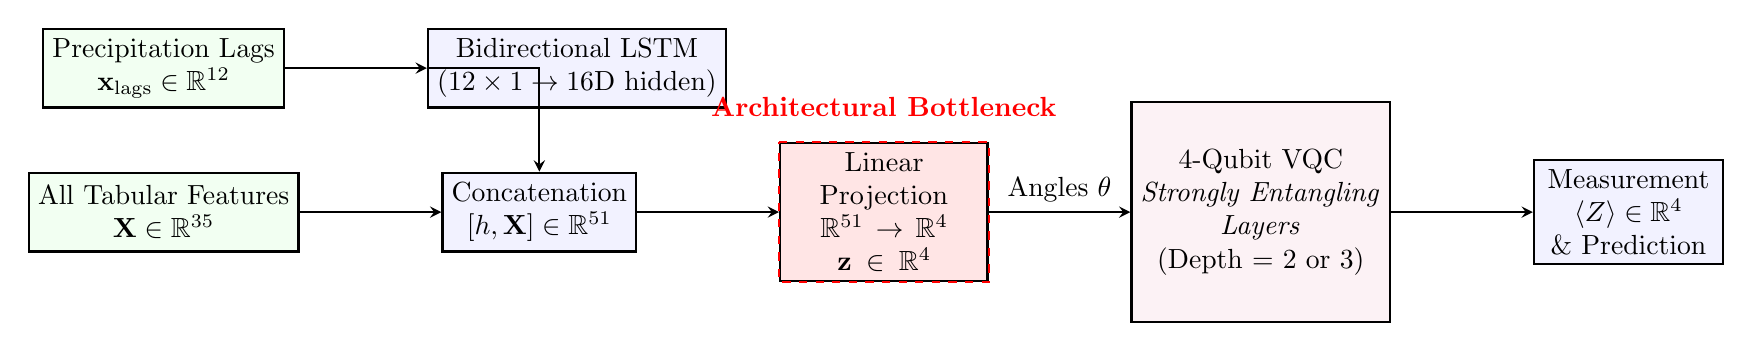
\begin{tikzpicture}[
        node distance=1.2cm and 1.8cm,
        box/.style={rectangle, draw=black, thick, minimum width=2.4cm, minimum height=1cm, align=center, fill=blue!5},
        quantum/.style={rectangle, draw=black, thick, minimum width=2.4cm, minimum height=2.8cm, align=center, fill=purple!5},
        arrow/.style={thick,->,>=stealth}
    ]
    \node (lags) [box, fill=green!5] {Precipitation Lags \\ $\mathbf{x}_{\text{lags}} \in \mathbb{R}^{12}$};
    \node (lstm) [box, right=of lags] {Bidirectional LSTM \\ ($12 \times 1 \to 16\text{D}$ hidden)};
    \node (features) [box, below=0.8cm of lags, fill=green!5] {All Tabular Features \\ $\mathbf{X} \in \mathbb{R}^{35}$};
    \node (concat) [box, right=of features] {Concatenation \\ $[h, \mathbf{X}] \in \mathbb{R}^{51}$};
    \node (bottleneck) [box, right=of concat, fill=red!10, text width=2.4cm] {Linear Projection \\ $\mathbb{R}^{51} \to \mathbb{R}^{4}$ \\ $\mathbf{z} \in \mathbb{R}^{4}$};
    \node (vqc) [quantum, right=of bottleneck] {4-Qubit VQC \\ \textit{Strongly Entangling} \\ \textit{Layers} \\ (Depth = 2 or 3)};
    \node (output) [box, right=of vqc] {Measurement \\ $\langle Z \rangle \in \mathbb{R}^4$ \\ \& Prediction};
    
    \draw [arrow] (lags) -- (lstm);
    \draw [arrow] (lstm) -| (concat);
    \draw [arrow] (features) -- (concat);
    \draw [arrow] (concat) -- (bottleneck);
    \draw [arrow] (bottleneck) -- node[above] {Angles $\theta$} (vqc);
    \draw [arrow] (vqc) -- (output);
    
    \draw[dashed, red, thick] (bottleneck.north west) -- (bottleneck.north east) -- (bottleneck.south east) -- (bottleneck.south west) -- cycle;
    \node[above=0.2cm of bottleneck, text=red, font=\bfseries] {Architectural Bottleneck};
    \end{tikzpicture}%
    }
    \caption{Hybrid Quantum-Classical Architecture. The bidirectional LSTM processes the univariate 12-month precipitation lag sequence ($\mathbf{x}_{\text{lags}} \in \mathbb{R}^{12}$), producing a 16-dimensional recurrent representation. This is concatenated with the full 35-dimensional tabular feature vector (which redundantly contains the 12 lags alongside physical covariates and station indicators) to form a 51-dimensional representation. A classical linear projection ($\mathbb{R}^{51} \to \mathbb{R}^4$) then compresses the features into 4 continuous rotation angles for encoding into the 4-qubit Variational Quantum Circuit.}
    \label{fig:architecture}
\end{figure}

\begin{figure}[htbp]
    \centering
    \resizebox{0.95\textwidth}{!}{%
    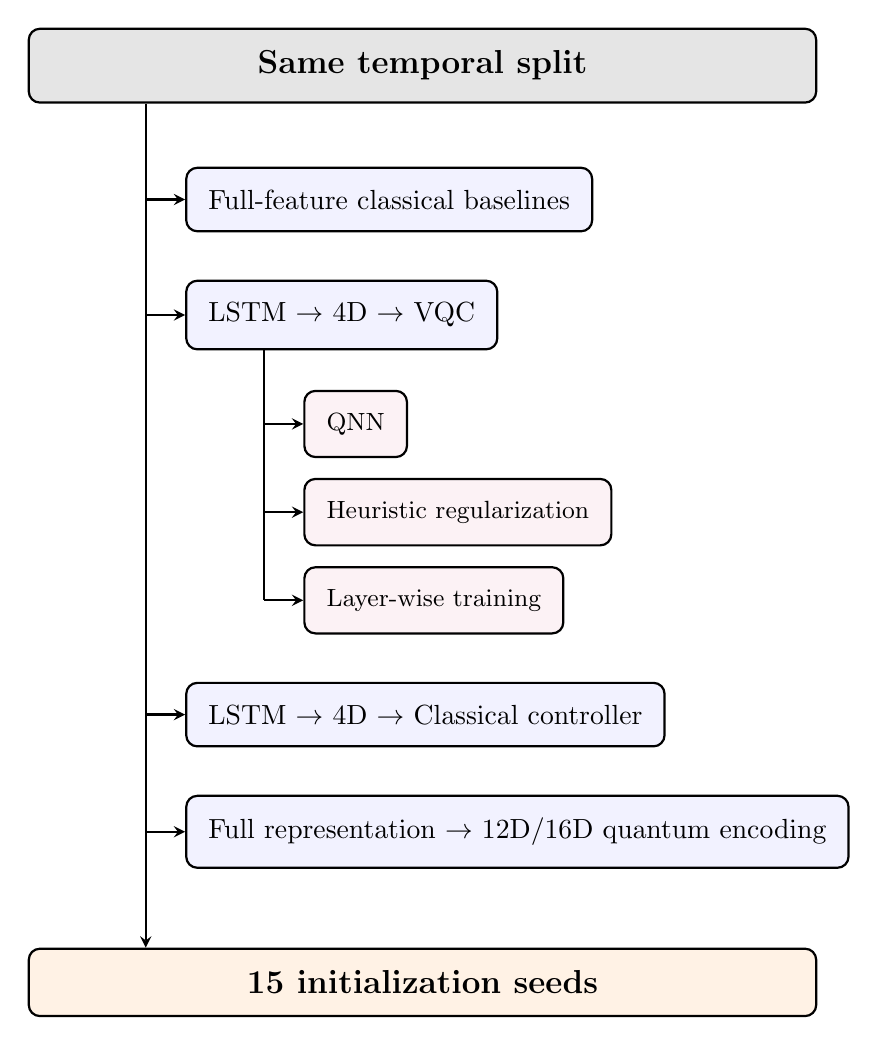
\begin{tikzpicture}[
        >=stealth,
        % Global node styles
        box/.style={rectangle, draw=black, thick, rounded corners, fill=white, inner sep=8pt, align=left, font=\normalsize},
        root/.style={box, fill=gray!20, font=\bfseries\large, align=center, minimum width=10cm},
        l1/.style={box, fill=blue!5},
        l2/.style={box, fill=purple!5, font=\small},
        seed/.style={box, fill=orange!10, font=\bfseries\large, align=center, minimum width=10cm}
    ]

    % ==========================================
    % 1. NODES DEFINITION
    % ==========================================
    
    % ROOT NODE
    \node[root] (split) {Same temporal split};

    % Define the X coordinate for the main vertical backbone
    \coordinate (L1_x) at ([xshift=1.5cm]split.south west);

    % LEVEL 1: Baselines
    \node[l1, anchor=north west] (class) at ([xshift=0.5cm, yshift=-0.8cm]L1_x) {Full-feature classical baselines};

    % LEVEL 1: VQC Base
    \node[l1, anchor=north west] (vqc) at ([yshift=-0.6cm]class.south west) {LSTM $\rightarrow$ 4D $\rightarrow$ VQC};

        % Define the X coordinate for the VQC sub-backbone
        \coordinate (VQC_branch) at ([xshift=1cm]vqc.south west);

        % LEVEL 2: VQC Branches
        \node[l2, anchor=north west] (qnn) at ([xshift=0.5cm, yshift=-0.5cm]VQC_branch |- vqc.south) {QNN};
        \node[l2, anchor=north west] (phys) at ([yshift=-0.25cm]qnn.south west) {Heuristic regularization};
        \node[l2, anchor=north west] (lbl) at ([yshift=-0.25cm]phys.south west) {Layer-wise training};

    % LEVEL 1: Classical Controller Control
    % We use (lbl.south -| class.west) to ensure it stays below the L2 nodes but aligns left with L1
    \node[l1, anchor=north west] (control) at ([yshift=-0.6cm]lbl.south -| class.west) {LSTM $\rightarrow$ 4D $\rightarrow$ Classical controller};

    % LEVEL 1: Bandwidth Extension
    \node[l1, anchor=north west] (enc) at ([yshift=-0.6cm]control.south west) {Full representation $\rightarrow$ 12D/16D quantum encoding};

    % BOTTOM NODE: Seeds
    % Centered relative to the root node
    \node[seed, anchor=north] (seeds) at ([yshift=-1cm]enc.south -| split.center) {15 initialization seeds};

    % ==========================================
    % 2. PATH DRAWING (ARROWS)
    % ==========================================

    % Main vertical backbone 
    \draw[thick] (L1_x) -- (L1_x |- enc.west);
    
    % The backbone continues down to hit the top of the 'seeds' box
    \draw[thick, ->] (L1_x |- enc.west) -- (L1_x |- seeds.north);

    % Horizontal branches to Level 1
    \draw[thick, ->] (L1_x |- class.west) -- (class.west);
    \draw[thick, ->] (L1_x |- vqc.west) -- (vqc.west);
    \draw[thick, ->] (L1_x |- control.west) -- (control.west);
    \draw[thick, ->] (L1_x |- enc.west) -- (enc.west);

    % VQC vertical sub-backbone
    \draw[thick] (VQC_branch) -- (VQC_branch |- lbl.west);
    
    % Horizontal branches to Level 2
    \draw[thick, ->] (VQC_branch |- qnn.west) -- (qnn.west);
    \draw[thick, ->] (VQC_branch |- phys.west) -- (phys.west);
    \draw[thick, ->] (VQC_branch |- lbl.west) -- (lbl.west);

    \end{tikzpicture}%
    }
    \caption{Schematic of the experimental design. All evaluated architectures use the same temporal split and are each trained with 15 initialization seeds to characterize optimization variance. The hierarchy separates the full-feature classical baselines from the hybrid quantum models, and pairs the latter with bottleneck-matched classical controls and encoding-bandwidth ablations.}
    \label{fig:experimental_design}
\end{figure}

To test whether domain-motivated soft constraints alter optimization trajectories, we evaluate two hybrid configurations incorporating heuristic thermodynamic regularization (\texttt{LSTM+PI-QNN} and \texttt{LbL-QNN}). As detailed in \Cref{app:heuristic_regularization}, this scheme supplements binary cross-entropy with two phenomenological soft penalties: a temperature-dependent gating term ($\mathcal{L}_{\text{CC}}$) penalizing high precipitation predictions under restricted saturation-capacity conditions, and a latent-coordinate balance term ($\mathcal{L}_{\text{hMSE}}$) acting on the 4-qubit expectation readout coordinates ($q_0, \dots, q_3$). These are empirical soft regularizers rather than first-principles thermodynamic conservation laws. As shown in \Cref{sec:stability}, the 15-seed replication shows no detected performance advantage of this heuristic regularization over the unconstrained hybrid baseline (descriptive Friedman diagnostic, $p = 0.458$).

\subsection{Quantum and Classical Architectures}
\label{app:architectures}

We evaluate ten distinct model architectures alongside one threshold-matched operational configuration (yielding eleven evaluation configurations in \Cref{tab:single_run_results}), grouped into four paradigms:
\begin{enumerate}
    \item \textbf{Statistical and Climatological Reference Baselines:} We evaluate non-parametric reference benchmarks alongside $L_2$-regularized Logistic Regression: (i) \emph{Month $\times$ Station Climatology}, which assigns each test sample the empirical frequency of precipitation exceeding $P_{60}$ observed for that specific station and calendar month in the training partition (AUC = 0.680, Brier score = 0.222, Brier skill score relative to the sample base rate = $+0.082$); and (ii) a binarized calendar-month climatology (training exceedance frequency per calendar month, pooled over stations), evaluated as an unranked binary baseline thresholded at 0.5 ($\text{Acc} = 64.58\%$, $\text{F1} = 0.522$, binary $\text{AUC} = 0.619$), whereas physical lag-1 precipitation persistence achieves $\text{AUC} = 0.589$.

    \item \textbf{Classical Ensembles:} Random Forest (300 estimators), Gradient Boosting (200 estimators), and XGBoost (500 estimators, depth=4).
    \item \textbf{Deep Learning Baselines:} A standalone bidirectional LSTM (\texttt{PureLSTM}) with 2 layers and 16 hidden units per direction (yielding a concatenated 32-dimensional sequence representation), concatenated with the 35 input features (67 dimensions), followed by batch normalization (\texttt{BatchNorm1d(67)}) and a two-layer classification head (\texttt{Linear(67, 16)} + LayerNorm + \texttt{Linear(16, 1)}), totaling 10,103 parameters, optimized using AdamW. Alongside this model, we evaluate \texttt{Matched LSTM}, an operational configuration of \texttt{PureLSTM} with its classification threshold adjusted to match the false positive rate of the hybrid models ($\tau = 0.531$; \Cref{app:operational_analysis}). The standalone LSTM is not capacity-matched to the hybrids (10,103 vs.\ $\sim$2,600 parameters; 16 vs.\ 8 hidden units per direction; batch normalization; and direct access to raw features without a 4-dimensional projection bottleneck).
    \item \textbf{Hybrid Quantum-Classical Models:} Developed using PennyLane's \texttt{default.qubit} simulator. \texttt{LSTM+QNN}, \texttt{LSTM+PI-QNN} and \texttt{LbL-QNN} use a bidirectional LSTM trained end to end (hidden dimension 8 per direction, 2,368 parameters) concatenated with the 35 input features to produce a 51-dimensional representation, which is compressed via a linear layer (\texttt{Linear(51, 4)}, 208 parameters) into a 4-dimensional projection bottleneck before being encoded into a 4-qubit Variational Quantum Circuit. The circuit uses a Strongly Entangling Layers ansatz with same-vector data re-uploading ($R_y$ and $R_z$ rotations per qubit repeated in each layer; \citealp{perez2020}) followed by parameterized $\mathrm{SU}(2)$ $\mathrm{Rot}$ gates and a circular CNOT entanglement topology ($L = 2$ layers with 24 quantum parameters for baseline models; $L = 3$ layers with 36 quantum parameters for the layer-wise \texttt{LbL-QNN} model; see \Cref{fig:vqc_circuit}). We distinguish this repeated encoding from the \emph{information-widening} re-uploading variant introduced later (\Cref{sec:relaxing_bottleneck}), which injects distinct feature subsets at each block.
    \begin{itemize}
        \item \texttt{LSTM+QNN}: Standard end-to-end unconstrained variational network (2 layers).
        \item \texttt{LSTM+PI-QNN}: End-to-end network optimized with the heuristic thermodynamic loss $\mathcal{L}_{\text{total}}$ (2 layers; \Cref{app:heuristic_regularization}).
        \item \texttt{LSTM+QTL}: Quantum Transfer Learning \citep{mari2020}, which differs in architecture from the three models above: the standalone \texttt{PureLSTM} (10,103 parameters, \Cref{tab:parameter_accounting}) is first trained as a classical model with early stopping and then frozen; its 32-dimensional state and the 35 features (67 dimensions) feed a trainable classical adapter ($67\rightarrow8\rightarrow4$), followed by a single angle encoding (RY, no re-uploading) and a 2-layer circuit. It has 617 trainable parameters, of which 24 are quantum.
        \item \texttt{LbL-QNN}\footnote{This architecture combines layer-by-layer training \citep{skolik2021} with the heuristic thermodynamic loss (\Cref{app:heuristic_regularization}). As shown in \Cref{app:depth_justification}, a depth-matched ablation specifically evaluating \texttt{LbL-QNN} against an end-to-end 3-layer architecture (\texttt{LSTM+PI-QNN-3L}) showed lower observed across-seed variability for the combined layer-wise configuration. However, this comparison is confounded by an expanded training budget (55 total epochs: 10 epochs per layer across 3 layers = 30 epochs, followed by 25 global fine-tuning epochs vs.\ 25 single-run epochs) and a staged learning rate schedule ($5\times 10^{-3}$ then $5\times 10^{-4}$ vs.\ fixed $5\times 10^{-3}$). The observed variance stabilization is therefore associated with the combined multi-stage schedule and expanded budget rather than demonstrably caused by the layer-wise inductive bias in isolation, particularly since a penalty-free layer-by-layer control and an epoch-matched (55-epoch) end-to-end control were not evaluated; the observed performance should be attributed to the combined layer-wise/heuristic configuration.}: applies the layer-by-layer training protocol to the \texttt{LSTM+PI-QNN} architecture, using a 3-layer circuit to support a non-degenerate three-stage freezing schedule.
        \item \texttt{QKSVM}: Quantum Kernel Support Vector Machine utilizing a Nystr\"{o}m approximation ($M=64$ landmarks) to handle the panel's size.
    \end{itemize}
\end{enumerate}

\begin{figure}[htbp]
    \centering
    \resizebox{\textwidth}{!}{%
    \begin{quantikz}[row sep=0.5cm, column sep=0.45cm]
        \lstick{$\ket{0}_{q_0}$} &
        \gategroup[wires=4, steps=2, style={dashed, rounded corners, fill=blue!5, inner sep=6pt}, background, label style={label position=above, anchor=south, yshift=0.2cm}]{\makebox[0pt]{Data Encoding}} \gate{R_y(x_0)} & \gate{R_z(x_0)} &
        \gategroup[wires=4, steps=5, style={dashed, rounded corners, fill=purple!5, inner sep=6pt}, background, label style={label position=above, anchor=south, yshift=0.2cm}]{\makebox[0pt]{Variational Ansatz}} \gate{\mathrm{Rot}(\vec\theta_0)} &
        \ctrl{1} & \qw & \qw & \targ{} & \meter{} \\
        \lstick{$\ket{0}_{q_1}$} & \gate{R_y(x_1)} & \gate{R_z(x_1)} & \gate{\mathrm{Rot}(\vec\theta_1)} & \targ{} & \ctrl{1} & \qw & \qw & \meter{} \\
        \lstick{$\ket{0}_{q_2}$} & \gate{R_y(x_2)} & \gate{R_z(x_2)} & \gate{\mathrm{Rot}(\vec\theta_2)} & \qw & \targ{} & \ctrl{1} & \qw & \meter{} \\
        \lstick{$\ket{0}_{q_3}$} & \gate{R_y(x_3)} & \gate{R_z(x_3)} & \gate{\mathrm{Rot}(\vec\theta_3)} & \qw & \qw & \targ{} & \ctrl{-3} & \meter{}
    \end{quantikz}%
    }
    \caption{Gate-level schematic of a single layer of the 4-qubit Variational Quantum Circuit
    (VQC). The 4-dimensional classical bottleneck vector $\mathbf{x}$ is injected into the quantum
    state via consecutive $R_y(x_i)$ and $R_z(x_i)$ rotations on each qubit (Data Encoding; \citealp{perez2020}). The trainable ansatz consists of general
    $\mathrm{SU}(2)$ rotations ($\mathrm{Rot}$ gates, each parameterized by a 3-component vector
    $\vec\theta_i = (\theta_{i,1}, \theta_{i,2}, \theta_{i,3})$) followed by a circular CNOT
    entanglement topology. To implement the Strongly Entangling Layers architecture, this entire
    encoding-ansatz block is repeated $L$ times (with $L=2$ for the baseline models, yielding 24 quantum parameters, and $L=3$ for
    the layer-wise \texttt{LbL-QNN} model, yielding 36 quantum parameters). Readout is performed via Pauli-$Z$ measurements on
    all qubits.}
    \label{fig:vqc_circuit}
\end{figure}

\section{Training Hyperparameters}
\label{app:hyperparams}
% ============================================================

The Core experiment uses the configuration of \Cref{tab:core_spec}; for the standalone LSTM, the architecture and training loop coincide with the historical configuration below, and \texttt{LSTM+PI-QNN}, \texttt{LbL-QNN} and \texttt{LSTM+QTL} use the hyperparameters of \Cref{tab:hyperparams}. \Cref{tab:hyperparams} reports the full hyperparameter configuration for all evaluated
architectures, to support exact reproducibility.

\begin{table}[htbp]
\centering
\caption{Training hyperparameters for all evaluated architectures. All gradient-optimized models
use identical early-stopping criteria (patience = 6 epochs monitoring BCE validation loss) unless
noted in \textit{Other}.}
\label{tab:hyperparams}
\setlength{\tabcolsep}{4pt}
\begin{tabularx}{\textwidth}{@{} l c c c c >{\raggedright\arraybackslash}X @{}}
\toprule
\textbf{Architecture} & \textbf{Optimizer} & \textbf{LR} & \textbf{Batch} & \textbf{Epochs} & \textbf{Other} \\
\midrule
Logistic Regression & L-BFGS & --- & --- & --- & L2 penalty, $C=0.1$ \\
Random Forest & --- & --- & --- & --- & 300 trees, max\_depth=8 \\
Gradient Boosting & --- & 0.05$^\ddagger$ & --- & --- & 200 est., subsample=1.0, max\_features=None \\
XGBoost & --- & 0.05$^\ddagger$ & --- & --- & 500 est., depth=4, subsample=0.8, colsample\_bytree=0.8, scale\_pos\_weight $= n_{\text{neg}}/n_{\text{pos}}$ \\
\midrule
Standalone LSTM & AdamW & 0.005 & 16 & 25 & 16 hidden units/direction (32D concat.), LSTM dropout=0.3, head dropout=0.2 \\
LSTM+QNN & AdamW & 0.005 & 16 & 25 & 4 qubits, 2 layers \\
LSTM+PI-QNN & AdamW & 0.005 & 16 & 25 & $\lambda_{cc}=0.2, \lambda_{\text{hMSE}}=0.1$ \\
LSTM+QTL & AdamW & 0.002 & 8 & 15 & frozen LSTM, patience=4 \\
LbL-QNN & AdamW & var.\textsuperscript{*} & 16 & 55\textsuperscript{**} & freeze: 10 eps/layer, pat=7 \\
LSTM+MLP-4D (Linear-20) & AdamW & 0.005 & 16 & 25 & Linear(4$\to$4), 20 params, exact structural parity \\
LSTM+MLP-4D (LeakyReLU-28) & AdamW & 0.005 & 16 & 25 & Linear(4$\to$2) + LeakyReLU + Linear(2$\to$2) + LeakyReLU + Linear(2$\to$4), 28 params, He init \\
LSTM+MLP-4D (GELU-180) & AdamW & 0.005 & 16 & 25 & Linear(4$\to$16) +GELU + LN(16) + Linear(16$\to$4), 180 params \\
\bottomrule
\end{tabularx}
\vspace{4pt}
\raggedright
{\footnotesize\textsuperscript{*} \texttt{LbL-QNN} uses $5 \times 10^{-3}$ during layer-wise
freezing and $5 \times 10^{-4}$ during global fine-tuning.\\
\textsuperscript{**} Total epoch budget: 10 epochs per frozen layer (3 layers) plus 25 epochs of
global fine-tuning.\\
\textsuperscript{$\ddagger$} For tree ensembles, ``LR'' denotes the boosting shrinkage parameter,
not a gradient-descent step size.\par}
\end{table}

The classical ensemble hyperparameters and the quantum penalty weights ($\lambda_{cc}$, $\lambda_{\text{hMSE}}$) were manually specified; a reproducible tuning history is unavailable. Matched human tuning effort does not equate to matched compute budgets \citep{bowles2024}, and equal tuning effort across model families should not be assumed. The variance differences documented in this paper were not isolated from tuning effort.

% ============================================================
\section{Heuristic Thermodynamic Regularization, Latent Coordinates, and Sensitivity Sweep}
\label{app:heuristic_regularization}\label{sec:physics_loss}
% ============================================================

\subsection{Formulation of Heuristic Thermodynamic Loss Penalties}
To explore whether domain-motivated soft constraints alter optimization behavior, we constructed two heuristic regularizers combining binary cross-entropy ($\mathcal{L}_{\text{BCE}}$) with physical penalties:
\begin{equation}
\mathcal{L}_{\text{total}} = \mathcal{L}_{\text{BCE}} + \alpha(e) \left[ \lambda_{\text{cc}} \mathcal{L}_{\text{CC}} + \lambda_{\text{hMSE}} \mathcal{L}_{\text{hMSE}} \right]
\end{equation}
where $\alpha(e) = \min(1.0, e / (0.6 \times E_{\text{total}}))$ represents a linear annealing schedule across training epochs $e$.

\textbf{1. Clausius--Clapeyron-Inspired Gating Penalty ($\mathcal{L}_{\text{CC}}$):} Defines a temperature-dependent soft gate:
\begin{equation}
C_{\text{CC}} = \exp(0.07 \cdot T_{\text{anomaly}} \cdot 10.0)
\end{equation}
loosely motivated by the exponential scaling of saturation water vapor pressure with temperature ($\approx 7\%/\unit{\kelvin}$). A ReLU-gated penalty activates if the model predicts high precipitation probability ($P_{\text{rain}} > 0.6$) when this thermal gate is restricted:
\begin{equation}
\mathcal{L}_{\text{CC}} = \frac{1}{N} \sum_{i=1}^N \left[ \max(0, P_{\text{rain}, i} - 0.6) \times \max(0, 1.0 - C_{\text{CC}, i}) \right]
\end{equation}

\textbf{Dimensional and Physical Caveat:} The scale factor $0.07$ originates as a per-kelvin physical sensitivity from the Clausius--Clapeyron relation, but in the implementation it is multiplied by $10.0$ (which implicitly scales a $1\sigma$ anomaly to $10$\,K, whereas monthly temperature anomalies in the panel are typically $\sim 1$--$2$\,K) and evaluated on an antecedent monthly anomaly rather than concurrent temperature during precipitation; moreover, \texttt{t\_anomaly} is standardized against the trailing 12 months and therefore largely tracks the seasonal cycle. Furthermore, the 3-month lagged thermal difference (\texttt{choque\_clausius}) reflects seasonal transition cooling rather than saturation thermodynamics, and mapping qubits $q_0, q_1, q_3$ to latent thermodynamic quantities is an empirical inductive design since the classical $51\to 4$ projection is unconstrained. Consequently, $C_{\text{CC}}$ and $\mathcal{L}_{\text{hMSE}}$ are heuristic regularizing constraints rather than dimensionally closed thermodynamic equations. The sign of the gate is also not validated: it penalizes high rain probabilities under cold antecedent anomalies, whereas heavy autumn precipitation in this region is often associated with cold air aloft over a warm sea.

\textbf{2. Heuristic Latent-Coordinate Balance Penalty ($\mathcal{L}_{\text{hMSE}}$):} Encourages the readout expectation values nominally associated with sensible heat ($q_0$) and latent heat ($q_1$) to balance the coordinate nominally associated with convective release ($q_3$):
\begin{equation}
\mathcal{L}_{\text{hMSE}} = \frac{1}{N} \sum_{i=1}^N \left[ \max(0, q_{0,i}) + \max(0, q_{1,i}) - \max(0, q_{3,i}) - 0.5 \right]^2
\end{equation}
where $q_j = \langle 0 | U^\dagger(\theta, x) \sigma_z^{(j)} U(\theta, x) | 0 \rangle$ denotes the expectation value of Pauli-$Z$ on qubit $j$. We use the notation $\mathcal{L}_{\text{hMSE}}$ to distinguish this heuristic coordinate penalty from standard regression Mean Squared Error.

The internal constants ($0.07$, $10.0$, $0.6$, $0.5$) and outer penalty weights ($\lambda_{\text{cc}} = 0.2$, $\lambda_{\text{hMSE}} = 0.1$) were set by hand, with no tuning protocol recorded, based on qualitative heuristic reasoning and held fixed during main benchmark training.

Physics-informed learning embeds domain constraints in the loss \citep{raissi2019,karniadakis2021}, including in quantum models \citep{jaderberg2024}; the penalties used here are a loose, heuristic version of that idea. Exact architectural symmetries, such as equivariant quantum neural networks \citep{meyer2023,nguyen2024}, are a more principled direction for physics-informed QML.

\subsection{Latent Readout Coordinate Interpretations}
\Cref{tab:qubits_mapping} details the descriptive interpretations heuristically assigned to the four Pauli-$Z$ readout expectations. These labels are descriptive post-hoc conventions and do not correspond to physical thermodynamic state variables or conservation laws.

\begin{table}[htbp]
\centering
\caption{Post-hoc interpretation of the four measured latent coordinates. The labels are descriptive only and do not imply thermodynamic units, state identification, or physically enforced energy conservation.}
\label{tab:qubits_mapping}
\begin{tabular}{lll}
\toprule
\textbf{Qubit} & \textbf{Latent Coordinate} & \textbf{Heuristic interpretation} \\
\midrule
$Q_0$ & Thermal Energy Coordinate ($q_0$) & Thermal-related latent coordinate \\
$Q_1$ & Moisture Coordinate ($q_1$) & Moisture-related latent coordinate \\
$Q_2$ & Dynamic Coordinate ($q_2$) & Dynamic-related latent coordinate \\
$Q_3$ & Convective Release Coordinate ($q_3$) & Convective-related latent coordinate \\
\bottomrule
\end{tabular}
\end{table}

% ============================================================
\section{Circuit and Computational Cost Analysis}
\label{app:computational_cost}
% ============================================================

This appendix provides the complete software environment specification (\Cref{tab:software_env}), native gate decomposition (\Cref{tab:circuit_gates}), hybrid parameter accounting (\Cref{tab:parameter_accounting}), dimensionality reduction costs (\Cref{tab:dim_reduction}), shot-based execution projections (\Cref{tab:shots_cost}), and total computational cost summary (\Cref{tab:cost_summary}) for all evaluated quantum architectures. All gate counts were verified via PennyLane 0.45 \texttt{QuantumTape} decomposition to native \{RY, RZ, CNOT\} gates.

\subsection{Software Environment and Hardware}

\begin{table}[htbp]
\centering
\caption{Software environment and simulation hardware.}
\label{tab:software_env}
\begin{tabular}{ll}
\toprule
\textbf{Component} & \textbf{Version/Specification} \\
\midrule
PennyLane & 0.45.0 \\
PyTorch & 2.11.0+cpu \\
Python & 3.12.0 (MSC v.1935 64-bit AMD64) \\
NumPy & 2.0.2 \\
Qiskit Aer & $\ge$0.17 (NISQ noise simulation) \\
\midrule
Simulator & \texttt{default.qubit} (PennyLane statevector) \\
Differentiation & \texttt{diff\_method='backprop'} (analytical, through statevector) \\
Hardware & CPU-only (\texttt{cpuonly} in environment.yml, \texttt{+cpu} in PyTorch build) \\
NISQ noise sim & \texttt{qiskit.aer} with depolarizing noise model, \texttt{shots=1024} \\
\bottomrule
\end{tabular}
\end{table}

\subsection{Circuit Architecture: Decomposed Gate Counts}

\begin{table}[htbp]
\centering
\caption{Circuit decomposition to native gates for all evaluated quantum architectures.}
\label{tab:circuit_gates}
\resizebox{\textwidth}{!}{%
\begin{tabular}{lcccccc}
\toprule
\textbf{Circuit} & \textbf{Qubits} & \textbf{Depth} & \textbf{Total Gates} & \textbf{Single-Qubit} & \textbf{CNOTs} & \textbf{Quantum Params} \\
\midrule
LSTM+QNN / PI-QNN (4q, 2L) & 4 & 18 & 48 & 40 & 8 & 24 \\
LbL-QNN (4q, 3L) & 4 & 27 & 72 & 60 & 12 & 36 \\
QTL (4q, 2L) & 4 & 13 & 36 & 28 & 8 & 24 \\
QKSVM kernel (4q) & 4 & 2 & 8 & 8 & 0 & 0 (data only) \\
\midrule
\multicolumn{7}{l}{\textit{Encoding-bandwidth ablation circuits}} \\
Amplitude Embedding (4q, 2L) & 4 & 27 & 50\textsuperscript{*} & 28 & 22 & 24 \\
Re-uploading-3$\times$4D (4q, 3L) & 4 & 27 & 72 & 60 & 12 & 36 \\
\bottomrule
\end{tabular}%
}
\vspace{2pt}
\raggedright
{\footnotesize\textsuperscript{*}Amplitude state-preparation gate count depends on the decomposition scheme and on the input: the 50 gates (12 RY, 16 RZ, 22 CNOT) and depth 27 were counted on one decomposed instance under PennyLane's default M\"ott\"onen state preparation, in which zero-angle rotations are pruned. Preparing a generic real 4-qubit state requires 15 RY rotations and 14 CNOTs, so the count is a lower bound. Circuit depths are compiled on the native gate set $\{RY, RZ, CNOT\}$ using PennyLane's DAG critical-path analysis.\par}
\end{table}

\textbf{Gate decomposition detail (LSTM+QNN, 4q-2L):} Per layer, the encoding block 
applies $4\times \text{RY} + 4\times \text{RZ} = 8$ single-qubit gates (data embedding via RY and RZ rotations). The 
\texttt{StronglyEntanglingLayers} block applies $4\times \text{Rot}(\theta,\phi,\omega) \rightarrow 
4\times \text{RY} + 8\times \text{RZ} + 4\times \text{CNOT} = 16$ gates. Totals for 2 layers: 
8 RY(data) + 8 RZ(data) + 8 RY(param) + 16 RZ(param) + 8 CNOT = \textbf{48 gates} (16 RY, 24 RZ, 8 CNOT). LbL-QNN adds a third block, totaling \textbf{72 gates} (24 RY, 36 RZ, 12 CNOT). QTL uses \textbf{36 gates} (12 RY, 16 RZ, 8 CNOT). Re-uploading-3$\times$4D uses 3 sequential encoding and entangling blocks, totaling \textbf{72 gates} (24 RY, 36 RZ, 12 CNOT). Compiled critical-path circuit depths on the native $\{RY, RZ, CNOT\}$ basis are 18 for LSTM+QNN / PI-QNN, 27 for LbL-QNN, 13 for QTL, 2 for QKSVM, 27 for Amplitude Embedding, and 27 for Re-uploading-3$\times$4D.

\subsection{Hybrid Model Parameter Accounting}

\begin{table}[htbp]
\centering
\caption{Complete parameter accounting for hybrid quantum-classical models. 
\texttt{in\_dim} = 35 for 4 stations (12 precipitation lags + 17 physics features + 2 seasonal + 4 station dummies).}
\label{tab:parameter_accounting}
\resizebox{\columnwidth}{!}{%
\begin{tabular}{lrrrr}
\toprule
\textbf{Model} & \textbf{Total Params} & \textbf{Trainable Params} & \textbf{Quantum (W)} & \textbf{Classical} \\
\midrule
LSTM+QNN (4q, 2L) & 2,613 & 2,613 & 24 & 2,589 \\
LSTM+PI-QNN (4q, 2L) & 2,613 & 2,613 & 24 & 2,589 \\
LbL-QNN (4q, 3L) & 2,625 & 2,625 & 36 & 2,589 \\
QTL (4q, 2L) & 10,720 & \textbf{617} & 24 & 593 (adapter+head) \\
PureLSTM (baseline) & 10,103 & 10,103 & --- & 10,103 \\
Amplitude Embedding (4q, 2L) & 3,237 & 3,237 & 24 & 3,213 \\
Re-uploading-3$\times$4D (4q, 3L) & 3,041 & 3,041 & 36 & 3,005 \\
\midrule
\multicolumn{5}{l}{\textit{Classical bottleneck controls}} \\
Linear parity control & 2,609 & 2,609 & 0 & 2,609 \\
LeakyMLP parity control & 2,617 & 2,617 & 0 & 2,617 \\
GELU MLP control & 2,769 & 2,769 & 0 & 2,769 \\
\bottomrule
\end{tabular}%
}
\end{table}

In LSTM+QNN, only 24/2,613 = \textbf{0.92\% of trainable parameters} 
are quantum. The circuit adds 48 gates on a 16-dimensional state vector atop a 2,589-parameter 
classical backbone (2,368-parameter LSTM encoder + 208-parameter projection layer + 13-parameter normalization and head). For QTL, the entire 
PureLSTM encoder (10,103 params) is frozen; only the adapter network (580 params) + head/norm (13 params) + quantum circuit 
weights (24 params) are trainable = 617 trainable parameters (3.89\% quantum).

\subsection{Dimensionality Reduction Cost}

The full input dimensionality is 35 (with 4 stations). Hybrid models concatenate the 16-dimensional bidirectional LSTM representation with the 35 raw features, yielding a 51-dimensional intermediate representation. The circuit operates on only 4 qubits; inside the models, a classical linear layer projects the 51-dimensional representation to 4 dimensions.

\begin{table}[htbp]
\centering
\caption{Dimensionality reduction pipeline and associated classical cost.}
\label{tab:dim_reduction}
\resizebox{\textwidth}{!}{%
\begin{tabular}{llll}
\toprule
\textbf{Model} & \textbf{Reduction Method} & \textbf{From $\rightarrow$ To} & \textbf{Params in Reduction} \\
\midrule
LSTM+QNN / PI-QNN & \texttt{nn.Linear(16 + in\_dim, n\_q)} & 51 $\rightarrow$ 4 & 51$\times$4 + 4 = \textbf{208} \\
QTL & \texttt{nn.Linear(67, 8)} $\rightarrow$ \texttt{nn.Linear(8, 4)} & 67 $\rightarrow$ 8 $\rightarrow$ 4 & 67$\times$8+8 + 8$\times$4+4 = \textbf{580} \\
QKSVM & PCA(\texttt{n\_components=4}) + MinMaxScaler & 35 $\rightarrow$ 4 & 0 trainable (eigendecomposition: $O(d^2 N + d^3)$) \\
Amplitude & \texttt{nn.Linear(16 + in\_dim, 2\^{}n\_q)} & 51 $\rightarrow$ 16 & 51$\times$16 + 16 = \textbf{832} \\
Re-uploading (3 blocks) & \texttt{nn.Linear(16 + in\_dim, 12)} & 51 $\rightarrow$ 12 & 12$\times$51 + 12 = \textbf{624} \\
\bottomrule
\end{tabular}%
}
\end{table}

The LSTM encoder before the projection compresses the 12 precipitation lags into a 16-dim 
hidden state (bidirectional LSTM, 2 layers, hidden=8), adding:
\begin{itemize}
    \item LSTM: \texttt{nn.LSTM(1, 8, 2, bidirectional=True)} $\rightarrow$ \textbf{2,368 parameters}
    \item The projection sees: \textbf{16 (LSTM hidden) + 35 (in\_dim)} $\rightarrow$ \textbf{51}
\end{itemize}

Including the full classical preprocessing (LSTM encoder + projection) 
means that most trainable parameters are classical. The circuit adds 48 gates 
on a 16-dimensional state vector atop a 2,589-parameter classical backbone; the parameter count alone does not quantify the functional contribution of the circuit.

\subsection{Circuit Evaluations and Computational Cost}

\subsubsection{Statevector mode (\texttt{diff\_method='backprop'})}

\begin{itemize}
    \item \textbf{Forward pass:} 1 circuit evaluation per sample
    \item \textbf{Backward pass:} no additional circuit executions (the gradient is obtained by backpropagation through 
    the statevector, which has its own cost)
    \item \textbf{Per epoch:} $N_{\text{train}}$ circuit evaluations (forward only)
    \item \textbf{Per training run (25 epochs):} $\le 25 \times N_{\text{train}}$
\end{itemize}

State vector size: $2^4 = 16$ complex amplitudes. Memory per state: $16 \times 16$ bytes 
(complex128) = 256 bytes for the basic statevector (excluding autograd storage). Backprop gradient cost: $O(2^n \times \text{depth})$ 
per sample. The 4-qubit statevector is small; the computational bottleneck is the sequential Python loop
over samples (no batching across samples in the quantum part).

\subsubsection{Estimated Cost With Shots (Hardware / Parameter-Shift)}

If running on real quantum hardware (parameter-shift rule instead of backprop):

\begin{table}[htbp]
\centering
\caption{Circuit evaluations per sample under parameter-shift rule with $N_{\text{shots}}=1024$.}
\label{tab:shots_cost}
{\small
\setlength{\tabcolsep}{5pt}
\begin{tabular}{lcc}
\toprule
\textbf{Component} & \textbf{LSTM+QNN (24 params)} & \textbf{LbL-QNN (36 params)} \\
\midrule
Forward & 1 circuit $\times$ 1024 shots & 1 circuit $\times$ 1024 shots \\
Backward (parameter-shift) & $2 \times 24 = 48$ circuits $\times$ 1024 shots & $2 \times 36 = 72$ circuits $\times$ 1024 shots \\
\textbf{Total per sample} & \textbf{49 circuits $\times$ 1024 shots} & \textbf{73 circuits $\times$ 1024 shots} \\
\textbf{Total shots per sample} & \textbf{50,176} & \textbf{74,752} \\
\bottomrule
\end{tabular}%
}
\end{table}

The table counts parameter-shift evaluations for the variational circuit weights only. It excludes the input-angle derivatives required for end-to-end training, execution overhead and hardware latency, and is not a measured runtime ratio relative to statevector backpropagation. Finite sampling adds shot noise.

\subsection{Summary: Gate, Parameter and Partial Execution-Count Profile}

\begin{table}[htbp]
\centering
\caption{Gate, parameter and partial execution-count summary for the quantum architectures (excludes runtime, input-angle derivatives and hardware overheads).}
\label{tab:cost_summary}
\resizebox{\textwidth}{!}{%
\begin{tabular}{lccccc}
\toprule
\textbf{Metric} & \textbf{LSTM+QNN} & \textbf{PI-QNN} & \textbf{LbL-QNN} & \textbf{QTL} & \textbf{QKSVM} \\
\midrule
Qubits & 4 & 4 & 4 & 4 & 4 \\
Circuit depth & 18 & 18 & 27 & 13 & 2 \\
Single-qubit gates & 40 & 40 & 60 & 28 & 8 \\
CNOTs & 8 & 8 & 12 & 8 & 0 \\
Total gates & 48 & 48 & 72 & 36 & 8 \\
Quantum params & 24 & 24 & 36 & 24 & 0 (fixed map) \\
Total trainable params & 2,613 & 2,613 & 2,625 & 617 & N/A (SVM) \\
Classical params & 2,589 & 2,589 & 2,589 & 593 & PCA+SVM \\
\textbf{\% quantum params} & \textbf{0.92\%} & \textbf{0.92\%} & \textbf{1.37\%} & \textbf{3.89\%} & \textbf{Fixed map\textsuperscript{*}} \\
Statevector cost & $O(16 \times \text{depth})$ & $O(16 \times \text{depth})$ & $O(16 \times \text{depth})$ & $O(16 \times \text{depth})$ & $O(16)$ \\
Shots cost ($N=1024$) & 49$\times$1024/sample & 49$\times$1024/sample & 73$\times$1024/sample & 49$\times$1024/sample & 1$\times$1024/kernel \\
Diff method & backprop & backprop & backprop & backprop & N/A \\
Simulator & default.qubit & default.qubit & default.qubit & default.qubit & default.qubit \\
Hardware & CPU (statevector) & CPU (statevector) & CPU (statevector) & CPU (statevector) & CPU (statevector) \\
Max epochs & 25 & 25 & 55 (30+25) & 15 & N/A \\
Dim. reduction & 51$\rightarrow$4 (linear) & 51$\rightarrow$4 (linear) & 51$\rightarrow$4 (linear) & 67$\rightarrow$4 (2-layer) & 35$\rightarrow$4 (PCA) \\
\bottomrule
\end{tabular}%
}
\vspace{2pt}
\raggedright
{\footnotesize\textsuperscript{*}QKSVM uses a fixed 4-qubit quantum feature map without variational parameters; optimization is classical quadratic programming in the dual space.\par}
\end{table}


% ============================================================
\section{Historical Runs in the Canonical Pipeline}
\label{app:historical}
% ============================================================

All results in this section come from the canonical pipeline (checkpoint \texttt{01\_data.pt}), in which the synoptic anomalies are standardized with the full 1938--2026 record and the scikit-learn tree ensembles are fitted on the 2,787 training and validation rows. These runs preceded the train-only pipeline of the main text. For most of them only per-seed AUCs, or the test probabilities of single runs (seed 42, and seed 0 regenerated for the hybrids), were archived, so no paired seed-mean intervals can be computed, and Random Forest and XGBoost were run with an earlier software environment. They are descriptive and are not used for the inferential claims of the main text. Random Forest, XGBoost, the standalone LSTM, the Linear-4D control and the four variational hybrids were re-run in the train-only pipeline with all test probabilities stored (\Cref{M-tab:case,M-tab:brier}); where a historical value below differs from the train-only one, the train-only value is the reference. The quantum-kernel SVM, logistic regression, gradient boosting, the bottleneck and bandwidth variants, the operational metrics and the noise and ablation analyses exist only in this canonical form.

\subsection{Hybrid Architectures and Further Comparisons}
\label{app:hybrids}

\Cref{tab:multiseed} gives the 15-seed AUC of the main models next to the climatology. Random Forest has the highest mean in every pipeline and every hybrid is below it. In the train-only Core experiment the four variational hybrids lie 0.020--0.026 below Random Forest, with paired intervals in \Cref{M-tab:qnn_paired,M-tab:hyb_paired}; the canonical-pipeline values are historical runs with seed-0 probabilities only, and their gaps to Random Forest (up to 0.033) are point estimates. The canonical Random Forest of 2{,}787 rows (0.6851) is the archived run (scikit-learn 1.6.1); the 2{,}273-row value (0.6802) was computed in scikit-learn 1.9.1, in which the 2{,}787-row model scores 0.6875, so the effect of the extra rows in the canonical pipeline is $+0.007$ and not the $+0.005$ obtained by subtracting the two table entries (script \path{exp20_rf_fitting_rows.py}). The train-only Random Forest labelled 2{,}787 rows in an earlier version of this table turned out to be the 2{,}273-row fit (\Cref{M-sec:validation_protocol}), and its row is removed.


\begin{table}[htbp]
\centering
\caption{15-seed test AUC, sorted by mean. Pipeline: TO = train-only anomaly standardization (re-run, primary); C = canonical pipeline. SD is the sample standard deviation ($n-1$). Last column: difference to the climatology (AUC 0.6796, shown as 0.680 elsewhere); it is a descriptive gap, not a test.}
\label{tab:multiseed}
{\small
\begin{tabular}{llccc}
\toprule
\textbf{Model} & \textbf{Pipeline} & \textbf{Mean AUC} & \textbf{SD} & \textbf{Gap to clim.} \\
\midrule
Random Forest (2,787 rows) & C & 0.6851 & 0.0026 & $+0.006$ \\
Random Forest (2,273 rows) & TO & 0.6829 & 0.0035 & $+0.003$ \\
Random Forest (2,273 rows) & C & 0.6802 & 0.0035 & $+0.001$ \\
Gradient Boosting & C & 0.6692 & 0.0022 & $-0.010$ \\
Reuploading-3$\times$4D & C & 0.6688 & 0.0085 & $-0.011$ \\
Standalone LSTM & TO & 0.6682 & 0.0063 & $-0.011$ \\
Standalone LSTM & C & 0.6657 & 0.0091 & $-0.014$ \\
Amplitude-16D & C & 0.6643 & 0.0114 & $-0.015$ \\
LSTM+QNN & TO & 0.6634 & 0.0098 & $-0.016$ \\
LbL-QNN & TO & 0.6632 & 0.0129 & $-0.016$ \\
XGBoost & TO & 0.662 & 0.0054 & $-0.018$ \\
LbL-QNN & C & 0.6605 & 0.0089 & $-0.019$ \\
LSTM+PI-QNN & TO & 0.6601 & 0.0170 & $-0.020$ \\
LSTM+QNN & C & 0.6589 & 0.0153 & $-0.021$ \\
XGBoost & C & 0.6575 & 0.0051 & $-0.022$ \\
LSTM+QTL & TO & 0.6565 & 0.0147 & $-0.023$ \\
LSTM+PI-QNN & C & 0.6555 & 0.0172 & $-0.024$ \\
Linear-4D control & TO & 0.6539 & 0.0078 & $-0.026$ \\
LSTM+QTL & C & 0.6519 & 0.0128 & $-0.028$ \\
Bottleneck-free LSTM (hidden 8) & C & 0.6435 & 0.0065 & $-0.036$ \\
\bottomrule
\end{tabular}%
}
\end{table}

\textbf{Single-run claims among hybrids.} In a single run, \texttt{LbL-QNN} reached an AUC of 0.672, tracking Random Forest (DeLong $p=0.2124$) and nominally above \texttt{LSTM+QNN} ($p=0.0070$) and the standalone LSTM (0.653, $p=0.0263$; the latter comparison is also confounded by the capacity mismatch). Across 15 seeds the means of \texttt{LbL-QNN} and \texttt{LSTM+QNN} are 0.6605 and 0.6589. Over the $15\times15=225$ seed pairs, \texttt{LbL-QNN} has the higher AUC in 52.0\,\% of cases and \texttt{LSTM+QNN} in 48.0\,\%, an almost symmetric distribution. A paired DeLong test on every seed pair would need the per-seed test probabilities, which were archived only for seed 0 in these canonical runs, so none is made; in the train-only Core experiment the two models have 15-seed means of 0.6632 and 0.6634 (\Cref{M-tab:case}). An omnibus Friedman test finds no difference among the four quantum models ($\chi^2(3)=2.600$, $p=0.458$, Kendall's $W=0.058$). These are seed-level statements; the sampling-error argument of \Cref{M-sec:budget} applies to them as well.

\textbf{Equivalence margins.} In the historical fixed-test seed-level analysis, GELU satisfied the $\pm0.010$ margin and the linear controller satisfied $\pm0.015$; LeakyReLU required $\pm0.020$ (for \texttt{LSTM+QNN} versus \texttt{LbL-QNN}: mean difference $-0.0016$, 90\,\% CI $[-0.0095,+0.0062]$, $p_{\text{TOST}}=0.041$ at $\pm0.010$). These tests use seed variance only, the margins were not justified by a scientific or practical criterion, and the paired structure of the seed index is a convention. They do not establish sampling-aware equivalence of predictive performance; a TOST that includes sampling error would require the per-seed test probabilities of these historical runs, which are not available (\Cref{app:multiseed,app:bottleneck}); for the train-only Core experiment the sampling-aware intervals are in \Cref{M-tab:qnn_paired,M-tab:hyb_paired}.

\textbf{Bottleneck-matched controls.} The end-to-end hybrids compress a 51-dimensional vector to 4 angles. Three classical controllers on the identical 4-dimensional interface (linear, 20 parameters; LeakyReLU, 28; GELU, 180) obtain AUC $0.6545$, $0.6516$ and $0.6563$ against $0.6589$ for \texttt{LSTM+QNN}, with Wilcoxon $p\in[0.17,0.64]$ (\Cref{app:bottleneck}). The gaps are 0.003--0.007 on the historical seed-level data. A bottleneck-free LSTM with the same hidden size scores lower ($0.6435\pm0.0065$) than the 4-dimensional controls, and full-feature XGBoost (0.662 train-only; 0.6575 in the canonical pipeline of the hybrids, \Cref{tab:multiseed}) is comparable to \texttt{LSTM+QNN} (0.659). The evidence therefore does not support the hypothesis that the 4-dimensional bottleneck is the cause of the gap between hybrids and tree ensembles: the data do not identify the bottleneck as its cause, and removing the bottleneck did not raise the score of the small recurrent backbone.

\textbf{Encoding bandwidth.} Widening the interface to 16D amplitude embedding or 12D data re-uploading gives AUC $0.6643$ and $0.6688$, i.e.\ 0.005--0.010 above \texttt{LSTM+QNN}. The Friedman test over six quantum models is nominally significant ($p=0.0228$, $W=0.174$), but the advantage of re-uploading over \texttt{LSTM+QNN} does not survive Holm correction ($p_{\text{Holm}}=0.083$), both variants use larger classical projection layers (832 and 624 weights, adding 624 and 416 parameters over the 4D bottleneck), and the re-uploading circuit is also deeper. Even the best bandwidth variant (re-uploading, 0.6688) stays 0.016 below Random Forest (0.6851), so the data neither show that wider encodings close the gap to the tree ensembles nor that they fail to. The paired sampling uncertainty required for an architecture-level conclusion was not reconstructed for these historical runs; the result is descriptive and exploratory (\Cref{app:bandwidth}).


\textbf{PCA-4 control for the quantum kernel.} Fitting a four-component PCA on the training partition only (65.7\,\% of the variance of the 35 features), a classical RBF-SVM reaches AUC 0.669 (Brier 0.2219) against 0.639 (0.2283) for the \texttt{QKSVM}. Random Forest and Gradient Boosting on the same four components score lower (0.631 $\pm$ 0.003 and 0.623 $\pm$ 0.0005). The 0.030 gap in favor of the classical kernel is descriptive: the paired standard error of this specific pair was not computed, so the result is consistent with, but does not establish, a disadvantage of the specific quantum feature map relative to classical kernels, and it suggests that low-dimensional compression alone does not explain the modest QKSVM score; a difference in effective kernel bandwidth between the two SVMs was not examined. We note that \texttt{QKSVM} uses an unentangled product-state AngleEmbedding without CNOT gates, so its fidelity kernel factorizes classically as $\prod_{j=1}^4 \cos^2((x_j - x'_j)/2)$ and does not evaluate an entangled quantum state space.



% ============================================================

\subsection{Single-Run Performance}
\label{sec:single_run}

We evaluate model performance on the canonical spatiotemporal test partition ($N=528$ station-months, 2008--2026) using the canonical dataset \texttt{01\_data.pt} ($P_{60}=28.1$, $P_{90}=86.32$\,mm). As established by the 15-seed rerun on the canonical dataset and the row-matched refits (\Cref{app:leakage_correction}), adopting a strict train-only standardization protocol moves the AUC by 0.003 or less with the fitting rows held fixed, with mixed sign across model families and without evidence of systematic leakage inflation.

\Cref{tab:single_run_results} summarizes the single-run test performance across all evaluated models at a fixed initialization seed (\texttt{seed=42}). Global accuracy is misleading due to class imbalance; we therefore focus on F1-score, ROC-AUC, and Precision-Recall AUC (PR-AUC; \citealp{davis2006,saito2015}). The tree-based \textbf{Random Forest} establishes the classical reference across ROC-AUC and F1 (AUC = 0.688, F1 = 0.603), while the non-parametric \textbf{Month $\times$ Station Climatology} establishes an empirical baseline that matches or exceeds all quantum models (AUC = 0.680, PR-AUC = 0.603). The hybrid quantum-classical architectures cluster tightly below (AUC: 0.639--0.672; F1: 0.580--0.604).

\begin{table}[htbp]
\centering
\caption{Comparative performance on the spatiotemporal test set (Single-Run), including Precision-Recall AUC (PR-AUC) alongside ROC-AUC. Single representative run evaluated at default threshold 0.5 ($n=20$ ACP-flagged test months exceeding $P_{60}$ out of 25 flagged total; $n=49$ $P_{90}$-exceeding test months). Month $\times$ Station Climatology establishes the non-parametric empirical baseline.}
\label{tab:single_run_results}
\setlength{\tabcolsep}{4.5pt}
\begin{tabular}{l c c c c c c c}
\toprule
\textbf{Model} & \textbf{Acc (\%)} & \textbf{F1} & \textbf{ROC-AUC} & \textbf{PR-AUC} & \textbf{Rc-$P_{90}$} & \textbf{Rc-ACP} & \textbf{FPR} \\
\midrule
\multicolumn{8}{l}{\textit{Climatological Reference}}\\
Month $\times$ Station Climatology & 61.2 & 0.547 & 0.680 & \textbf{0.603} & 0.653 & 0.600 & 0.360 \\
\midrule
\multicolumn{8}{l}{\textit{Statistical \& Ensemble}}\\
Logistic Regression & 62.3 & 0.472 & 0.655 & 0.546 & 0.571 & 0.650 & 0.228 \\
Random Forest & 63.8 & 0.603 & \textbf{0.688} & 0.591 & 0.755 & 0.900 & 0.383 \\
Gradient Boosting & 61.6 & 0.522 & 0.671 & 0.577 & 0.592 & 0.700 & 0.312 \\
XGBoost & 59.1 & 0.548 & 0.650 & 0.545 & 0.694 & 0.850 & 0.418 \\
\midrule
\multicolumn{8}{l}{\textit{Deep Learning}}\\
Standalone LSTM & 54.5 & 0.585 & 0.653 & 0.587\textsuperscript{*} & 0.816 & 0.950 & 0.617 \\
Matched LSTM$^{\dagger}$ & 57.2 & 0.565 & 0.653 & 0.587\textsuperscript{*} & 0.776 & 0.950 & 0.502 \\
\midrule
\multicolumn{8}{l}{\textit{Quantum-Classical Hybrid}}\\
LSTM+QNN & 58.0 & 0.599 & 0.639 & 0.504 & 0.796 & 0.950 & 0.550 \\
LSTM+PI-QNN & 58.9 & 0.583 & 0.662 & 0.558 & 0.755 & 0.950 & 0.489 \\
LSTM+QTL & 58.7 & 0.604 & 0.651 & 0.518 & 0.837 & 0.850 & 0.537 \\
\textbf{LbL-QNN} & 59.1 & 0.589 & 0.672 & 0.581 & 0.796 & 0.900 & 0.495 \\
QKSVM & 59.8 & 0.475 & 0.639 & 0.510 & 0.612 & 0.600 & 0.293 \\
\bottomrule
\end{tabular}
\vspace{4pt}

{\footnotesize
\textsuperscript{*}PR-AUC is threshold-independent and therefore identical to the unmatched Standalone LSTM row; only the operational point (FPR, recall) changes under matching.\par
\textsuperscript{$\dagger$}Threshold-recalibrated variant of Standalone LSTM, evaluated at an operating point matched in false-detection rate to \texttt{LbL-QNN} ($\tau = 0.531$); defined and motivated in \Cref{app:operational_analysis}.\par
Rc-ACP is evaluated strictly over the $n=20$ positive test months ($y=1$) matching the Autumn Convective Proxy in the canonical pipeline (out of 25 flagged months total), distinct from the 32 flagged months (25 positive) identified under train-only anomaly standardization (\Cref{app:leakage_correction}); if all 25 flagged months are counted regardless of precipitation (the alarm rate), the respective values are: Climatology 0.640, Logistic Regression 0.600, Random Forest 0.880, Gradient Boosting 0.680, XGBoost 0.840, Standalone LSTM 0.960, Matched LSTM 0.960, LSTM+QNN 0.920, LSTM+PI-QNN 0.960, LSTM+QTL 0.840, LbL-QNN 0.920, QKSVM 0.520.
}
\end{table}

In this single realization, the layer-wise hybrid \texttt{LbL-QNN} achieves the highest quantum AUC (0.672), tracking Random Forest (\Cref{tab:single_run_results}) with no statistically significant difference under an uncorrected DeLong test \citep{delong1988} ($p = 0.2124$; formal equivalence not tested). It nominally outperforms unconstrained \texttt{LSTM+QNN} ($p = 0.0070$) and \texttt{Standalone LSTM} ($p = 0.0263$), though the latter comparison is heavily confounded by the capacity mismatch (10,103 vs.\ $\sim$2,600 parameters; \Cref{M-sec:architectures}).

The single-run ordering does not withstand closer examination. First, formal paired testing against Month $\times$ Station Climatology was conducted on the leading model, Random Forest, yielding no statistically significant advantage under a paired DeLong test (point difference $\Delta \text{AUC} = +0.0079$, $\text{SE} = 0.0138$, $z = 0.578$, $p = 0.5635$) or a year-block bootstrap (mean of the bootstrap differences $+0.0068$, $95\%$ block CI: $[-0.0171, +0.0284]$, $p = 0.5420$). Because all evaluated quantum architectures and neural baselines achieved lower point AUCs and higher Brier scores than Random Forest, neither Random Forest nor any evaluated quantum architecture demonstrates statistically verifiable predictive skill beyond empirical seasonal-geographic climatology when temporal autocorrelation is respected.

Second, disaggregating test performance across individual monitoring stations reveals that the pooled ROC-AUC ($N=528$) aggregates disparate regional regimes. In Alicante ($N=221$, $29.4\%$ positive rate), Random Forest achieves an AUC of 0.698 and \texttt{LbL-QNN} achieves 0.683, compared to 0.681 for Climatology. In Barcelona ($N=221$, $50.2\%$ positive rate), Climatology achieves an AUC of 0.663, outperforming both Random Forest (0.634) and all quantum models (\texttt{LbL-QNN}: 0.643; \texttt{LSTM+QNN}: 0.538). In Valencia ($N=50$, $56.0\%$ positive rate), Climatology (0.692) likewise exceeds Random Forest (0.690), \texttt{LbL-QNN} (0.649), and \texttt{LSTM+QNN} (0.607), while in San Javier ($N=36$, $36.1\%$ positive rate), all models cluster between 0.535 and 0.575. This suggests that part of the pooled discriminative performance arises from separating high-base-rate from low-base-rate stations rather than dynamically resolving extreme months within a station regime.

Third, because the extreme tail contains limited test observations ($n=20$ ACP months exceeding $P_{60}$, $n=49$ $P_{90}$ months), point estimates of extreme recall carry wide 95\% Wilson confidence intervals (which ignore temporal and spatial dependence, and whose overlap is not a paired test of equality) that broadly overlap across all architectures (e.g., Random Forest $0.900$ [0.699, 0.972] vs.\ \texttt{LSTM+QNN} $0.950$ [0.764, 0.991]; documented in \Cref{app:operational_analysis}). Fourth, the apparent operational difference between \texttt{Standalone LSTM} (Rc-ACP = 0.950, FPR = 0.617) and \texttt{LbL-QNN} (Rc-ACP = 0.900, FPR = 0.495) is largely explained by the default threshold: recalibrating the classical LSTM to operate at an identical FPR of $\approx$50.2\% (\texttt{Matched LSTM}, $\tau = 0.531$) preserves its recall at 0.950 (19/20) with no statistically significant difference under paired bootstrap resampling ($n=2{,}000$; full analysis in \Cref{app:operational_analysis}). Finally, these single-run margins are not reproduced across seeds (\Cref{sec:stability}), so they do not indicate robust architectural advantages.

\subsection{Probabilistic Verification, Calibration, and Spatiotemporal Block Resampling}
\label{sec:calibration_and_block_bootstrap}

Because extreme-precipitation forecasting is intrinsically probabilistic, threshold-dependent binary metrics must be supplemented by proper scoring rules and calibration diagnostics. Across the test partition ($N_{\text{test}}=528$), the non-parametric Month $\times$ Station Climatology establishes a competitive reference Brier score of $0.2224$ (Brier Skill Score $\text{BSS}_{\text{uncond}} = +0.0816$ relative to the unconditional training base rate $0.4017$, $\text{BS}_{\text{uncond}} = 0.2422$, the Brier score on the test rows of the constant forecast equal to the training base rate; the test prevalence is 0.411, so this value differs from $\pi(1-\pi)=0.2403$ at $\pi=0.4017$). Among trained models, Random Forest and Gradient Boosting achieve the lowest probability error (Random Forest: $\text{BS} = 0.2230$, $\text{BSS}_{\text{uncond}} = +0.0791$; Gradient Boosting: $\text{BS} = 0.2236$, $\text{BSS}_{\text{uncond}} = +0.0767$), closely matching empirical climatology. Logistic Regression ($\text{BS} = 0.2258$, Expected Calibration Error $\text{ECE} = 0.0418$) and \texttt{QKSVM} ($\text{BS} = 0.2283$, $\text{ECE} = 0.0511$) achieve lower calibration error than neural baselines, though these models yield negative Brier skill relative to empirical climatology ($\text{BSS}_{\text{clim}} \in [-0.003, -0.027]$). In contrast, all variational hybrid architectures, the standalone LSTM and XGBoost (trained with class weighting, \texttt{scale\_pos\_weight}; Brier score $0.2471$, $\text{ECE}=0.126$) exhibit substantially larger calibration error in the archived single-run evaluation ($\text{ECE} \in [0.112, 0.149]$; Brier scores between $0.2352$ for \texttt{LbL-QNN} and $0.2536$ for \texttt{LSTM+QNN}), resulting in markedly worse skill scores relative to climatology ($\text{BSS}_{\text{clim}} \in [-0.058, -0.140]$). The 15-seed train-only evaluation of the main text (\Cref{M-tab:brier}) agrees: Random Forest matches the climatology on average and the other models are worse.

\begin{table}[htbp]
\centering
\caption{Single-run AUC and Brier score of the ten models against the month$\times$station climatology (canonical single run, seed 42; 528 test rows). BSS$_{\text{clim}} = 1-\text{BS}/0.2224$. Historical version of \Cref{M-tab:brier}.}
\label{tab:brier_single_run}
{\small
\begin{tabular}{lccc}
\toprule
\textbf{Model} & \textbf{AUC} & \textbf{Brier score} & \textbf{BSS}$_{\text{clim}}$ \\
\midrule
Month$\times$Station Climatology & 0.680 & 0.2224 & 0 \\
\midrule
Random Forest & 0.688 & 0.2230 & $-0.003$ \\
Gradient Boosting & 0.671 & 0.2236 & $-0.005$ \\
Logistic Regression & 0.655 & 0.2258 & $-0.015$ \\
XGBoost & 0.650 & 0.2471 & $-0.111$ \\
Standalone LSTM & 0.653 & 0.2438 & $-0.096$ \\
\midrule
QKSVM & 0.639 & 0.2283 & $-0.027$ \\
LbL-QNN & 0.672 & 0.2352 & $-0.058$ \\
LSTM+PI-QNN & 0.662 & 0.2376 & $-0.068$ \\
LSTM+QTL & 0.651 & 0.2460 & $-0.106$ \\
LSTM+QNN & 0.639 & 0.2536 & $-0.140$ \\
\bottomrule
\end{tabular}%
}
\end{table}

Furthermore, because standard DeLong tests assume sample independence that may be compromised by temporal autocorrelation, we conducted a year-block bootstrap analysis ($B = 2{,}000$ resamples of the 19 test calendar years 2008--2026; \citealp{kunsch1989}). When entire calendar years are resampled across all monitoring stations, the block interval excludes zero for Random Forest against \texttt{LbL-QNN} ($\Delta \text{AUC} = +0.0151$, $95\%$ block CI: $[+0.0007, +0.0281]$, $p = 0.0400$), whereas the DeLong test of the same pair does not ($p = 0.2124$), and for Random Forest against Standalone LSTM ($\Delta \text{AUC} = +0.0350$, $95\%$ block CI: $[+0.0183, +0.0501]$, $p = 0.0010$). These are single-seed comparisons: the seed-to-seed spread of the same models (\Cref{M-sec:budget}) is of the order of the gaps reported. The contrast with the seed-mean comparisons of the main text changes both the training realization and the preprocessing pipeline and therefore does not isolate initialization effects. Meanwhile, Gradient Boosting shows no statistically significant difference from \texttt{LbL-QNN} under block resampling ($\Delta \text{AUC} = -0.0010$, $95\%$ block CI: $[-0.0335, +0.0315]$, $p = 0.9280$).


\subsection{Feature Importance and Station Indicators}

\label{sec:feature_importance}

To understand how classical ensembles exploit the feature space, we analyze feature importances across model families. For Random Forest, evaluating Gini feature importance (Mean Decrease in Impurity, MDI) reveals that physically derived thermodynamic features account for $53.8\%$ of total model importance (led by seasonal thermal contrast \texttt{choque\_clausius} at $6.4\%$, cumulative evapotranspiration \texttt{et0\_sum} at $5.3\%$, and temperature anomaly \texttt{t\_anomaly} at $3.7\%$). Antecedent precipitation lags contribute $37.1\%$, cyclic month encodings account for $5.3\%$, and geographic station indicator dummies contribute only $3.8\%$. In contrast, XGBoost gain assigns greater weight to station-specific geographic indicators and cyclic month encodings, followed by thermodynamic proxies.

At face value, the high ranking of geographic indicators in boosted trees might suggest classical ensembles owe their advantage specifically to geographic fixed effects unavailable to the dimension-constrained quantum bottleneck. We test this directly via a station-identity ablation and the capacity-spanning classical control (\Cref{sec:bottleneck_control}), and describe the results descriptively: in a single-seed exploratory ablation, removing the station indicators did not degrade classical performance (\Cref{app:spatial_ablations}), and a classical network restricted to the same 4-dimensional bottleneck had a mean AUC close to that of the quantum circuit. Impurity-based importance does not identify a causal contribution. A plausible reading is that classical ensembles use the full \emph{high-dimensional} feature space---thermodynamic, moisture-lag and seasonal signals---rather than geographic information specifically (we note, however, that removing explicit station indicator dummies does not eliminate geographic information entirely, as station-dependent levels of covariates such as mean pressure \texttt{pmed} or temperature range remain available to the models). This describes what the tree ensembles use; it does not establish that compression causes the gap to the hybrids (\Cref{M-sec:applying}).

\subsection{The 15-Seed Replication of the Quantum Tier}
\label{sec:stability}\label{app:multiseed}

To test the stability of the single-run findings, we replicated the training pipeline across 15
independent random-parameter initialization seeds for all gradient-optimized architectures,
using the same seed indices 0--14. For the PyTorch-based quantum and deep-learning
architectures, seed $i$ is passed to a common \texttt{torch.manual\_seed} call; we did not verify that this yields identical minibatch order across architectures, so the seed index is treated as a label and not as a pairing device. For cross-paradigm comparisons against the scikit-learn-based classical ensembles
(\Cref{sec:classical_multiseed}), seed $i$ instead denotes a consistent nominal block index
rather than a mechanically shared random stream. \Cref{tab:quantum_multiseed,tab:operational_multiseed} present the resulting distributions for the quantum tier.

An omnibus Friedman test reveals no statistically significant difference in discriminative power
among the four quantum architectures ($\chi^2(3) = 2.600$, $p = 0.458$). The effect size is
small (Kendall's $W = 0.058$; \citealp{demsar2006}). The seed index is a label rather than a pairing device (see above), so the Friedman test is a descriptive diagnostic of the archived per-seed AUCs, not an inferential test. The single-run AUC
of 0.672 for \texttt{LbL-QNN} lies above its 15-seed mean of 0.6605. Pairwise Wilcoxon tests indicate that \texttt{LbL-QNN} is not
statistically superior to any unconstrained counterpart ($p \ge 0.547$ in all cases); notably,
unconstrained \texttt{LSTM+QNN} achieves the best mean rank of the four (2.200), with
\texttt{LbL-QNN} second (2.400). The ranks are computed within each seed across the four models, whereas the mean AUC averages the raw values, so a model with a few high-AUC seeds can have the higher mean (\texttt{LbL-QNN}, 0.6605 versus 0.6589) without the better mean rank; both differences are negligible against the noise.

To determine whether the absence of a statistically significant difference corresponds to
statistical equivalence, we conducted paired Two One-Sided Tests (TOST;
\citealp{schuirmann1987,lakens2017}) on seed-level AUC differences. For each model pair, let
\(d_i = \mathrm{AUC}_{A,i} - \mathrm{AUC}_{B,i}\) denote the paired difference across the
\(n=15\) initialization seeds indexed 0--14 (the index is a label, so the paired test is a descriptive diagnostic). We tested \(H_{01}:\mu_d\le-\Delta\) and
\(H_{02}:\mu_d\ge+\Delta\) using one-sided paired \(t\)-tests at \(\alpha=0.05\), with
\(\Delta=\pm0.010\) AUC as the reference margin. The numerical TOST criterion was satisfied when both null
hypotheses were rejected, equivalently when the paired \(90\%\) confidence interval for the
mean difference \(\bar d\) lay entirely within \((-\Delta,+\Delta)\). The margin was
defined before conducting the equivalence analysis but was not preregistered;
\(\Delta=\pm0.015\) and \(\pm0.020\) are reported as sensitivity analyses. Because the pairing is conventional and the margins lacked a practical justification, no equivalence claim is drawn from these calculations; they do not establish equivalence of generalization to new periods or stations. For \texttt{LSTM+QNN} versus \texttt{LbL-QNN},
the mean difference is \(-0.0016\) (with standard error \(\text{SE}_\Delta = 0.0045\), standard deviation of the paired difference \(\text{SD}_\Delta = 0.0173\), and paired seed correlation \(r \approx 0.05\)), with a paired \(90\%\) CI of
\([-0.0095,+0.0062]\) contained within the \(\pm0.010\) bounds
(\(p_{\mathrm{TOST}}=0.0407\)). Under sensitivity margins \(\Delta = \pm 0.015\) and \(\pm 0.020\), the margin is also satisfied at the wider margins (\(p_{\text{TOST}} \le 0.0028\)). These tests concern seed-level optimization only: test-set sampling uncertainty is far larger (standard error of one AUC 0.023--0.027; \Cref{M-sec:budget}), and the results do not establish sampling-aware equivalence.

To describe how often one seed outcome exceeds another, we analyzed the complete pairwise cross-seed comparison matrix ($15 \times 15 = 225$ pairs) between \texttt{LbL-QNN} and \texttt{LSTM+QNN}. Across all 225 realizations, \texttt{LbL-QNN} yields a higher test AUC than \texttt{LSTM+QNN} in 52.0\% of cases (117/225), whereas \texttt{LSTM+QNN} is higher in 48.0\% of cases (108/225)---a virtually symmetric distribution. Per-seed test probabilities of these canonical runs were archived only for seed 0, so no paired DeLong test is made on the 225 pairs; the 15-seed means of the two models differ by only 0.0016.

The clearest secondary pattern emerging from the quantum tier is lower across-seed variability
for the combined layer-wise/heuristic configuration. A depth-matched control for
\texttt{LbL-QNN} (\texttt{LSTM+PI-QNN-3L}) indicates that this variance reduction is not
explained by circuit depth alone (Levene's test at matched 3-layer depth,
$F_{\text{Levene}} = 7.47$, $p=0.011$; full analysis in
\Cref{app:depth_justification}). Because a penalty-free layer-wise control was not evaluated,
the separate contributions of the layer-by-layer protocol, the heuristic penalty, and the
expanded training budget remain not fully identified by the present design. The multi-seed
replication provides no evidence that heuristic thermodynamic regularization lowers the
false-alarm rate: the mean FPR of \texttt{LbL-QNN} ($0.541 \pm 0.079$) shows no statistically
significant difference from the unconstrained \texttt{LSTM+QNN} ($0.531 \pm 0.083$; Wilcoxon
$p = 0.847$).

\begin{table}[htbp]
\centering
\caption{Global AUC distribution across 15 independent training-seed replications (quantum models
only), sorted descending by mean AUC. Standard deviation is the sample standard deviation ($n-1$ denominator).}
\label{tab:quantum_multiseed}
\begin{tabular}{lcccc}
\toprule
\textbf{Architecture} & \textbf{Mean AUC} & \textbf{Std. Dev.} & \textbf{Minimum} & \textbf{Maximum} \\
\midrule
LbL-QNN & 0.6605 & 0.0089 & 0.645 & 0.681 \\
LSTM+QNN & 0.6589 & 0.0153 & 0.628 & 0.681 \\
LSTM+PI-QNN & 0.6555 & 0.0172 & 0.605 & 0.673 \\
LSTM+QTL & 0.6519 & 0.0128 & 0.632 & 0.679 \\
\bottomrule
\end{tabular}
\end{table}


\begin{table}[htbp]
\centering
\caption{Operational metric distributions (mean $\pm$ across-seed sample standard deviation, ddof=1) across 15 training seeds at a default decision threshold of 0.5, for all gradient-optimized and ensemble architectures ($n=20$ ACP months exceeding $P_{60}$, $n=49$ $P_{90}$ months).}
\label{tab:operational_multiseed}
\begin{tabular}{lccc}
\toprule
\textbf{Architecture} & \textbf{FPR} & \textbf{Rc-ACP} & \textbf{Rc-$P_{90}$} \\
\midrule
\textit{Classical Ensembles}\\
Random Forest & $0.383 \pm 0.011$ & $0.867 \pm 0.041$ & $0.746 \pm 0.022$ \\
Gradient Boosting & $0.310 \pm 0.006$ & $0.700 \pm 0.000$ & $0.595 \pm 0.007$ \\
XGBoost & $0.408 \pm 0.013$ & $0.890 \pm 0.047$ & $0.706 \pm 0.024$ \\
\midrule
\textit{Deep Learning}\\
Standalone LSTM & $0.513 \pm 0.066$ & $0.910 \pm 0.081$ & $0.782 \pm 0.031$ \\
\midrule
\textit{Quantum-Classical Hybrid}\\
LSTM+QNN & $0.531 \pm 0.083$ & $0.877 \pm 0.068$ & $0.785 \pm 0.047$ \\
LSTM+PI-QNN & $0.531 \pm 0.048$ & $0.897 \pm 0.079$ & $0.796 \pm 0.052$ \\
LSTM+QTL & $0.489 \pm 0.075$ & $0.860 \pm 0.069$ & $0.762 \pm 0.050$ \\
LbL-QNN & $0.541 \pm 0.079$ & $0.867 \pm 0.070$ & $0.784 \pm 0.045$ \\
\bottomrule
\end{tabular}
\vspace{4pt}

{\footnotesize Rc-ACP is evaluated strictly on the $n=20$ positive test months ($y=1$) matching the Autumn Convective Proxy in the canonical pipeline (25 flagged total), distinct from the 32 flagged months (25 positive) under train-only standardization (\Cref{app:leakage_correction}).}
\end{table}

\textit{Note on operational variance:} Across-seed variance in FPR is substantially higher in
gradient-optimized models (LSTMs and quantum hybrids) than in stochastic tree ensembles. Per-architecture across-seed standard deviations are given in \Cref{app:variance_decomposition}; they are descriptive and suggest that single-run operational comparisons among gradient-based models are unstable.

\subsection{Robustness of the Classical Reference}
\label{sec:classical_multiseed}

Extending the 15-seed replication to the classical baselines (\Cref{tab:multiseed}) shows that the \emph{direction} of the classical-over-quantum gap is consistent across seeds, whereas its size is not separated from test-sampling uncertainty by these seed-level data (\Cref{M-sec:budget}). Tree-based ensembles exhibit markedly lower across-seed variance ($\sigma_{\text{AUC}} \le 0.0054$) than the hybrid quantum architectures ($\sigma_{\text{AUC}} \in [0.0089, 0.0172]$ in \Cref{tab:multiseed}; classical neural baselines range from $0.0063$ for standalone LSTM to $0.0069$--$0.0083$ for 4D controllers).

An omnibus Friedman test across the eight canonical-pipeline architectures (Random Forest on 2,787 rows, Gradient Boosting, XGBoost, the standalone LSTM and the four hybrids) nominally reveals a significant overall ranking effect ($\chi^2(7) = 53.47$, $p < 10^{-6}$; Kendall's $W = 0.509$). However, because Friedman's test formally assumes commensurate, exchangeable blocks across all conditions, treating nominal seed indices across disparate software ecosystems (scikit-learn Mersenne Twister vs.\ PyTorch/PennyLane PRNG) as paired blocks should be regarded as a heuristic diagnostic rather than an exact inferential test. As a descriptive summary of optimization outcomes, across all 225 cross-framework seed pairs Random Forest (2,787 rows: $0.6851 \pm 0.0026$; the training-row-matched 2,273-row model scores $0.6802 \pm 0.0035$ in a different scikit-learn version) has a higher AUC than \texttt{LbL-QNN} in 224 of 225 pairs ($\hat{P} = 0.9956$, Cliff's $\delta = 0.9911$, the difference between the probabilities that a draw from one model exceeds a draw from the other and the reverse; \citealp{cliff1993}) and exceeds all other neural and quantum architectures in all pairs (complete matrix in \Cref{app:operational_analysis}). These cross-seed summaries describe optimization outcomes on the fixed historical test set. They are not independent replications of generalization performance and do not replace the paired sampling analyses in the main text. However, this optimization-seed separation on a fixed chronological split must not be mistaken for test-set generalization certainty: on the test partition itself, an uncorrected single-run DeLong test comparing Random Forest to \texttt{LbL-QNN} yields $p = 0.2124$, and the year-block bootstrap test against empirical climatology yields $p = 0.5420$, indicating that test-set sampling uncertainty ($N=528$ correlated station-months) remains substantial.



\subsection{Relaxing the Encoding Bottleneck}
\label{sec:relaxing_bottleneck}\label{app:bandwidth}

To test whether the 4D projection bottleneck constrains quantum performance, we evaluated two
bandwidth-widened architectures: Amplitude Embedding (16D) and Data Re-uploading (12D across 3
blocks), both projecting \emph{independently and directly} from the full 51-dimensional
pre-bottleneck representation---not from an expansion of the pre-existing 4D projection
(\Cref{app:encoding_architectures}; \citealp{perez2020}), following \Cref{tab:bottleneck_relaxation}.

A descriptive Friedman diagnostic across all six quantum architectures (seed index as a label, not a verified pairing) gives a nominal effect
($\chi^2(5)=13.057$, $p=0.0228$; $W=0.174$), markedly larger than the trivial effect size among
the original four ($W=0.058$; \Cref{sec:stability}). Both bandwidth-widened architectures achieve
the best mean ranks. However, Holm-Bonferroni correction \citep{holm1979} shows that
the nominal advantage of Reuploading-3$\times$4D over baseline \texttt{LSTM+QNN} ($p=0.0413$) does not
survive multiplicity adjustment ($p_{\text{Holm}}=0.0826$); and Amplitude-16D shows no statistically significant differentiation from baseline \texttt{LSTM+QNN} ($p=0.1688$). Furthermore, both widened configurations introduce $\sim 600$--$800$ classical parameters in the linear projection head, expanding total model capacity. Only Reuploading's advantage over
\texttt{LbL-QNN} survives ($p_{\text{Holm}}=0.006$), though that comparison confounds
re-uploading with \texttt{LbL-QNN}'s distinct training protocol and depth.

The widened variants had lower mean test AUC than Random Forest in these historical runs (canonical pipeline, matched 2,273 rows: $0.6802 \pm 0.0035$; 2,787 rows: $0.6851 \pm 0.0026$; \Cref{tab:bottleneck_relaxation}). Because the comparisons differ in architecture, projection size, depth and training conditions, and sampling-aware paired intervals were not reconstructed, these results do not establish whether widening the encoding interface changes the generalization gap. While Re-uploading-3$\times$4D exceeds the Standalone LSTM ($0.6657 \pm 0.0091$) and Amplitude-16D approaches it, the bottleneck-matched classical controls (\Cref{sec:bottleneck_control}) show no detectable circuit effect over classical linear/MLP projections at a fixed interface, and full-feature XGBoost ($0.6575 \pm 0.0051$) performs comparably to baseline \texttt{LSTM+QNN} ($0.6589 \pm 0.0153$). The Re-uploading architecture's improvement is also confounded
with an increase in circuit depth relative to the 2-layer \texttt{LSTM+QNN} baseline, so it cannot
be attributed to encoding bandwidth alone (unlike \texttt{LbL-QNN}, where a depth-matched 3-layer control was evaluated, the separate depth-matched control needed to disentangle these factors for re-uploading was not evaluated; see \Cref{M-sec:limitations}). We therefore report this result
descriptively, as evidence that widening the encoding interface is \emph{associated with} improved
relative standing among the evaluated quantum architectures, without concluding that bandwidth
alone drives the improvement. 

\begin{table}[htbp]
\centering
\caption{Global AUC distribution across 15 seeds for the encoding-bandwidth experiments, alongside
the original quantum architectures and the classical reference, sorted by mean rank.}
\label{tab:bottleneck_relaxation}
\begin{tabular}{lccc}
\toprule
\textbf{Architecture} & \textbf{Mean AUC} & \textbf{Std. Dev.} & \textbf{Mean Rank (of 6)} \\
\midrule
Reuploading-3$\times$4D & 0.6688 & 0.0085 & 2.333 \\
Amplitude-16D & 0.6643 & 0.0114 & 2.933 \\
LSTM+QNN & 0.6589 & 0.0153 & 3.600 \\
LSTM+PI-QNN & 0.6555 & 0.0172 & 3.733 \\
LbL-QNN & 0.6605 & 0.0089 & 3.800 \\
LSTM+QTL & 0.6519 & 0.0128 & 4.600 \\
\midrule
\textit{Random Forest (matched, 2,273 rows)}\textsuperscript{*} & \textit{0.6802} & \textit{0.0035} & --- \\
\textit{Random Forest (train+val, 2,787 rows)} & \textit{0.6851} & \textit{0.0026} & --- \\
\bottomrule
\end{tabular}
\vspace{4pt}

{\footnotesize\textsuperscript{*}Sensitivity baseline trained strictly on 2,273 rows.}
\end{table}

% ============================================================
% ============================================================
\subsection{Bottleneck-Controlled Classical Baseline}
\label{sec:bottleneck_control}\label{app:bottleneck}

A central confound in comparing hybrid quantum architectures against full-feature classical
ensembles is that the VQC-based models operate on a 4-dimensional projection produced by the LSTM
bottleneck, whereas classical ensembles ingest the full 35-dimensional engineered feature space,
including geographic fixed effects.

To isolate this confound, we evaluate three bottleneck-matched classical control configurations
(\texttt{LSTM+MLP-4D}) spanning a range of parameter counts. These architectures are identical to
\texttt{LSTM+QNN} in their upstream feature extractor, 4-dimensional projection bottleneck, and
downstream classification head, but replace the 4-qubit VQC with a classical controller (linear,
LeakyReLU, or GELU MLP). All configurations were replicated across the same 15 seed-indexed
initializations used for \texttt{LSTM+QNN} (\Cref{tab:bottleneck_control}). An initial width-2 ReLU-based control collapsed to
chance-level output (AUC$=0.500$) in 9 of 15 seeds due to dead-unit failure; we resolved this with
the linear and LeakyReLU configurations reported below, which is consistent with an
activation-specific rather than capacity-related failure (full diagnostic in \Cref{app:relu_collapse}).

Parameter count is a coarse and imperfect proxy for functional capacity: a
linear model and a nonlinear, GELU-activated MLP with comparable parameter counts are not
necessarily comparable in expressive power, since capacity depends jointly on activation
nonlinearity and architecture, not on parameter count alone. We therefore describe these three
controls as spanning a range of parameter counts and architectural nonlinearities, rather than as
strictly bottleneck-controlled to the quantum circuit in a formal sense. The qualitative conclusion
below does not depend on this caveat, because the absence of a statistically significant difference from the quantum
circuit holds independently for both the least expressive (linear) and most expressive (GELU)
control considered.

\begin{table}[htbp]
\centering
\caption{Bottleneck-controlled comparison: classical controls versus the quantum circuit under an
identical 4-dimensional information bottleneck, versus the full-feature Random Forest reference,
sorted descending by mean AUC. All values are 15-seed distributions with seed-indexed initialization (the index is a label, not a pairing device).}
\label{tab:bottleneck_control}
{\small
\setlength{\tabcolsep}{4.5pt}
\begin{tabular}{lcccc}
\toprule
\textbf{Architecture} & \textbf{Controller params} & \textbf{Mean AUC} & \textbf{Std. Dev.} & \textbf{Max} \\
\midrule
Random Forest (train+val, 2,787 rows)\textsuperscript{*} & Ensemble & 0.6851 & 0.0026 & 0.690 \\
Random Forest (matched, 2,273 rows)\textsuperscript{*} & Ensemble & 0.6802 & 0.0035 & 0.687 \\
LSTM+QNN (quantum, 4-dim. bottleneck) & 24 & 0.6589 & 0.0153 & 0.681 \\
GELU MLP (classical control, 4-dim. input) & 180 & 0.6563 & 0.0071 & 0.6725 \\
Linear (classical control, 4-dim. input) & 20 & 0.6545 & 0.0069 & 0.6680 \\
LeakyReLU MLP (classical control, 4-dim. input) & 28 & 0.6516 & 0.0083 & 0.6636 \\
\bottomrule
\end{tabular}%
}
\vspace{4pt}

{\footnotesize\textsuperscript{*}Tree ensemble capacity is determined by the number of leaves/nodes rather than differentiable parameters; the 300-tree Random Forest with \texttt{max\_depth=8} and the hybrid belong to different function classes and are not capacity-matched. The 2,273-row model provides the strictly matched training comparison to the neural and hybrid models. Parameter counts reported under Controller params reflect only the 4-dimensional controller/neck replacing the quantum circuit; for total model parameter accounting (including the shared 2,589 classical backbone), see \Cref{tab:parameter_accounting}.}
\end{table}

A 4-qubit circuit with 24 variational parameters operates on a state space of dimension $2^4 = 16$; its statevector evolution is represented by a $16 \times 16$ unitary matrix, which is classically simulable by statevector methods. Parameterized quantum circuits with angle encoding compute truncated Fourier series of the input coordinates \citep{schuld2021fourier}; classical models with trigonometric activations could therefore be functional analogues, but this was not tested here. 

As a historical fixed-test seed-level diagnostic (canonical pipeline), we conducted Two One-Sided Tests (TOST) against \texttt{LSTM+QNN} across the 15 seeds. Under a reference margin of $\Delta = \pm 0.010$ AUC, \texttt{GELU MLP-4D} satisfies the margin ($\text{Diff} = -0.0025$, paired 90\% CI $[-0.0092, +0.0041]$, $p_{\text{TOST}} = 0.0350$). The smaller \texttt{Linear-4D} ($\text{Diff} = -0.0044$, 90\% CI $[-0.0121, +0.0032]$, $p_{\text{TOST}} = 0.1113$) and \texttt{LeakyReLU-4D} ($\text{Diff} = -0.0073$, 90\% CI $[-0.0151, +0.0005]$, $p_{\text{TOST}} = 0.2772$) do not reject the $\pm 0.010$ margin. However, under a sensitivity margin of $\Delta = \pm 0.015$ AUC, \texttt{Linear-4D} also satisfies the margin ($p_{\text{TOST}} = 0.0148$), and \texttt{LeakyReLU-4D} requires $\Delta = \pm 0.020$ AUC ($p_{\text{TOST}} \le 0.0064$ for all three controllers). Wilcoxon signed-rank tests similarly show no significant differentiation ($p \in [0.17, 0.64]$), and do not detect a circuit effect at the fixed 4-dimensional interface. As in \Cref{M-sec:applying}, these seed-level tests omit test-set sampling error; they do not establish sampling-aware equivalence of predictive performance, and all three paired 90\% intervals lie within $\pm 0.016$ AUC.

We additionally evaluated classical controls under an unsupervised 4-dimensional compression of the entire 35-dimensional input space, providing an information-matched benchmark for \texttt{QKSVM} (\Cref{M-sec:architectures}). Fitting Principal Component Analysis strictly on the training partition ($\text{PCA}(4)$, capturing 65.70\% of total variance across the 35 features) and evaluating on the test partition, a classical Support Vector Machine with an RBF kernel achieves an AUC of 0.6686 and a Brier score of 0.2219 (with $\text{Acc} = 62.31\%$, $\text{F1} = 0.5158$, and $\text{Rc-ACP} = 0.8500$). This classical 4-dimensional benchmark outperforms the 4-qubit Quantum Kernel SVM (AUC = 0.6390, Brier score = 0.2283; \Cref{tab:single_run_results}) by 0.030 AUC (a descriptive gap; its paired sampling uncertainty was not computed), whereas tree ensembles on PCA-4 achieve lower discriminative performance (Random Forest: $0.6312 \pm 0.0030$; Gradient Boosting: $0.6230 \pm 0.0005$). This indicates that the modest score of \texttt{QKSVM} is not explained by low-dimensional compression alone; whether it reflects the inductive bias of the evaluated quantum feature map is not established by these data.

Random Forest is not a bottleneck-matched comparator for the VQC; it operates on the uncompressed 35-dimensional space with 300 trees, establishing an empirical tabular reference (canonical pipeline: mean AUC $= 0.6802 \pm 0.0035$ on matched 2,273 rows, scikit-learn 1.9.1; archived $0.6851 \pm 0.0026$ on 2,787 rows, scikit-learn 1.6.1). The 4D controls hold the input interface constant, isolating circuit-specific effects from representation compression: at this fixed interface, the historical seed-level means of the controllers lie within about 0.007 AUC of the hybrid. Restricting models to a 4D interface degrades performance relative to Random Forest, but the 4D controls show no detectable circuit effect at that interface. That full-feature XGBoost ($0.6575 \pm 0.0051$) scores close to baseline \texttt{LSTM+QNN} ($0.6589 \pm 0.0153$) shows that access to all features does not by itself guarantee a higher AUC; it does not show whether the bottleneck limits the hybrid. The residual gap to Random Forest may reflect model-family capabilities on tabular data rather than an encoding bottleneck, and was not tested here.

As exploratory evidence on whether the 4-dimensional compression itself constrains the recurrent backbone, we also evaluated a bottleneck-free classical LSTM with the same hidden dimension 8 (\texttt{bottleneck\_free\_lstm}, arithmetically $\sim$2,522 parameters: 2,368 LSTM + 102 BatchNorm + 52 linear head, though parameter counts were not stored in the checkpoint). Unlike the hybrid, which projects the 51-dimensional representation (16D LSTM hidden + 35D raw features) down to 4 dimensions before classification, this model attaches a direct linear classification head to the 51-dimensional vector. Across 15 seeds, it achieves an AUC of $0.6435 \pm 0.0065$. Because the classifier head differs and no paired seed-by-seed test was logged, this exploratory result does not support a claim that removing the bottleneck formally confirms compression as a performance limit. Descriptively, the bottleneck-free model falls below both the 4D linear control ($0.6545 \pm 0.0069$) and the 4D MLP controls ($0.6563 \pm 0.0071$, $0.6516 \pm 0.0083$), as well as the larger Standalone LSTM ($0.6657 \pm 0.0091$). That the 4D linear control scores 0.011 above the unprojected 51D head (a descriptive gap) at most suggests that low-dimensional linear projection can act as a regularizer for this small recurrent backbone, rather than compression acting solely as an upper bound on performance. We explicitly separate the claim of projection regularization from the claim that quantum circuits provide an inductive advantage at that interface.

The training protocol reveals an important asymmetry between model families: tree ensembles (Random Forest, Gradient Boosting, and XGBoost) were originally fit on the 2,787 rows of the combined training and validation partitions ($X_{\text{sk}} = X_{\text{all}}[:s_2]$), whereas neural and hybrid quantum models were fit on the 2,273 training rows with validation rows reserved for early stopping (\Cref{M-sec:validation_protocol}). Evaluating Random Forest strictly on the 2,273 training rows with canonical hyperparameters yields a 15-seed mean AUC of $0.6802 \pm 0.0035$ (range $[0.6732, 0.6867]$), compared to $0.6875 \pm 0.0044$ on 2,787 rows in the same software environment (scikit-learn 1.9.1; the archived 2,787-row run, scikit-learn 1.6.1, gives $0.6851 \pm 0.0026$). An automated Optuna search (50 trials) on the 2,273 training rows yielded $0.6798 \pm 0.0045$. In the train-only pipeline, which is primary in the main text, Random Forest is fitted on the same 2,273 training rows as the neural models, so the comparisons of the main text are not affected by this asymmetry; the extra validation rows would add 0.003 AUC there (\Cref{M-sec:validation_protocol}).


% ============================================================
\subsection{Encoding-Bandwidth Architectures}
\label{app:encoding_architectures}
Both extension architectures use separate projection layers mapping the 51-dimensional
pre-bottleneck representation $\mathbf{\tilde{h}}_t \in \mathbb{R}^{51}$ (16D LSTM hidden state
concatenated with the 35D raw engineered feature vector) directly to higher-dimensional spaces,
independently of and in parallel to the baseline architectures' own 4D projection head:
\begin{enumerate}
    \item \textbf{Amplitude Embedding:} Maps $\mathbf{\tilde{h}}_t$ to $\mathbf{z} \in
    \mathbb{R}^{16}$ via a dedicated linear layer. The state is prepared as
    $|\psi\rangle = \sum_{i=0}^{15} z_i |i\rangle$, with $\sum |z_i|^2 = 1$.
    \item \textbf{Data Re-uploading:} Maps $\mathbf{\tilde{h}}_t$ to $\mathbf{\theta} \in
    \mathbb{R}^{12}$ via a dedicated linear layer, partitioned into three disjoint 4-dimensional
    subsets injected sequentially as rotation angles across the three VQC layers.
\end{enumerate}

\subsection{Activation-Specific Collapse in Narrow Classical Bottlenecks}
\label{app:relu_collapse}
During development of the narrow MLP control, 9 of 15 seeds collapsed to constant prediction
(AUC = 0.500). This was diagnosed as a dead-ReLU pathology, where all hidden nodes fall into
negative pre-activation regimes during random initialization from $\mathcal{N}(0, \sigma^2)$.
Replacing ReLU with LeakyReLU (slope = 0.01) and He initialization, or using a bare linear layer,
removed the collapse in all 15 seeds, suggesting that the pathology was associated with the activation or its initialization rather than with capacity (activation and initialization were changed together). The quantum module does not contain ReLU units; this does not imply immunity of the hybrid model to degenerate predictions or optimization failure.

\subsection{Layer-by-Layer Depth Justification}
\label{app:depth_justification}
The \texttt{LbL-QNN} model uses a 3-layer circuit to facilitate a non-degenerate freezing
schedule across three training stages \citep{skolik2021}. To separate the effect of the
LbL protocol from the confounding effect of circuit depth, we additionally trained a depth-matched
control, \texttt{LSTM+PI-QNN-3L}: an end-to-end (non-frozen) 3-layer circuit, replicated across
the same 15 seeds.

Depth alone (2-layer $\to$ 3-layer, both end-to-end) produced no statistically significant change
in either variance (Levene's test \citep{levene1960}, $F_{\text{Levene}}=0.16$, $p=0.693$) or mean AUC (Wilcoxon, $p=0.208$) in this historical comparison. The depth-matched comparison showed lower observed across-seed variability for the combined layer-wise training configuration ($\sigma=0.0089$ vs.\ $\sigma=0.0154$; Levene's test, $F_{\text{Levene}}=7.47$, $p=0.011$; mean AUC Wilcoxon $p=0.073$). The design does not isolate layer-wise scheduling from the penalty, training duration and learning-rate changes: an unpenalized layer-by-layer control and an epoch-matched (55-epoch) end-to-end control were not evaluated.

The originally reported comparison between \texttt{LbL-QNN} and the
2-layer \texttt{LSTM+PI-QNN} baseline ($\sigma=0.0089$ vs.\ $\sigma=0.0171$)---which conflates
both depth and protocol---does not reach significance under a formal Levene's test
($F_{\text{Levene}}=1.80$, $p=0.191$) despite the descriptive point-estimate gap. The lower seed variance of the combined
\texttt{LbL-QNN} configuration is therefore observed in the depth-matched comparison above, not in
the uncontrolled 2-layer-vs-3-layer comparison, and it is not attributable to layer-wise training alone.

\subsection{Exploratory Analysis of Extreme-Tail and Operational Metrics}
\label{app:operational_analysis}
% ============================================================

\subsubsection{Small-Sample Binomial Uncertainty in Extreme-Tail Recall}
To evaluate model sensitivity in the extreme precipitation tail, the benchmark reports recall metrics conditioned on two diagnostic subsets: months exceeding the regional 90th percentile ($P_{90} = \qty{86.32}{\milli\meter}$, $n=49$ test months) and months matching the Autumn Convective Proxy (ACP, $n=25$ test months, of which 20 exceeded $P_{60}$; throughout this paper, Rc-ACP is defined over the $n=20$ months with $y=1$).

Given these small test-partition sample sizes, point estimates of Rc-ACP and Rc-$P_{90}$ carry substantial binomial sampling uncertainty. \Cref{tab:recall_wilson_ci} reports 95\% Wilson score confidence intervals \citep{wilson1927} for each evaluated architecture in the single representative run. As shown in the table, apparent single-run separations fall well within overlapping confidence intervals. For example, Random Forest's Rc-ACP ($0.900$, 95\% CI $[0.699, 0.972]$) and \texttt{LSTM+QNN}'s ($0.950$, 95\% CI $[0.764, 0.991]$) overlap substantially despite a 5-percentage-point difference in the point estimate, underscoring that single-run recall comparisons in the extreme tail reflect test-sample binomial uncertainty independent of optimization variability.

\begin{table}[htbp]
\centering
\caption{Extreme-tail recall with 95\% Wilson confidence intervals, single representative run ($n=20$ ACP-flagged test months exceeding $P_{60}$ out of 25 flagged total; $n=49$ $P_{90}$-exceeding test months).}
\label{tab:recall_wilson_ci}
\begin{tabular}{lcc}
\toprule
\textbf{Architecture} & \textbf{Rc-ACP [95\% CI]} & \textbf{Rc-$P_{90}$ [95\% CI]} \\
\midrule
\multicolumn{3}{l}{\textit{Climatological Reference}}\\
Month $\times$ Station Climatology & 0.600 [0.387, 0.781] & 0.653 [0.513, 0.771] \\
\midrule
\textit{Statistical \& Ensemble}\\
Logistic Regression & 0.650 [0.433, 0.819] & 0.571 [0.433, 0.699] \\
Random Forest & 0.900 [0.699, 0.972] & 0.755 [0.619, 0.854] \\
Gradient Boosting & 0.700 [0.481, 0.855] & 0.592 [0.452, 0.718] \\
XGBoost & 0.850 [0.640, 0.948] & 0.694 [0.555, 0.805] \\
\midrule
\textit{Deep Learning}\\
Standalone LSTM & 0.950 [0.764, 0.991] & 0.816 [0.686, 0.900] \\
Matched LSTM$^{\dagger}$ & 0.950 [0.764, 0.991] & 0.776 [0.641, 0.870] \\
\midrule
\textit{Quantum-Classical Hybrid}\\
LSTM+QNN & 0.950 [0.764, 0.991] & 0.796 [0.664, 0.885] \\
LSTM+PI-QNN & 0.950 [0.764, 0.991] & 0.755 [0.619, 0.854] \\
LSTM+QTL & 0.850 [0.640, 0.948] & 0.837 [0.710, 0.915] \\
LbL-QNN & 0.900 [0.699, 0.972] & 0.796 [0.664, 0.885] \\
QKSVM & 0.600 [0.387, 0.781] & 0.612 [0.472, 0.736] \\
\bottomrule
\end{tabular}
\vspace{4pt}

{\footnotesize\textsuperscript{$\dagger$}Threshold-recalibrated variant of Standalone LSTM ($\tau = 0.531$) matched to the false-detection rate of \texttt{LbL-QNN}.\par Rc-ACP is evaluated strictly on the $n=20$ positive test months ($y=1$) matching the Autumn Convective Proxy in the canonical pipeline (25 flagged total), distinct from the 32 flagged months (25 positive) under train-only standardization (\Cref{app:leakage_correction}).}
\end{table}

\subsubsection{Threshold Dependence of Operational Metrics}
At the default classification threshold of 0.5, the \texttt{Standalone LSTM} achieves high sensitivity to extremes (Rc-ACP = 0.950, 19/20) but has a high false-positive rate (FPR = 0.617). In contrast, \texttt{LbL-QNN} appears more conservative (FPR = 0.495, Rc-ACP = 0.900, 18/20), suggesting an apparent operational advantage for the hybrid architecture (\Cref{tab:single_run_results}).

However, this apparent advantage is sensitive to the selected operating threshold. When the classical LSTM is adjusted to operate at an approximately matched FPR of $\approx$50.2\% (versus 49.5\%) (by raising its decision threshold to $\tau = 0.531$, denoted \texttt{Matched LSTM}; $\tau$ was chosen on the test set to match the FPR, so this is a retrospective exploratory comparison and not an evaluation of a decision rule calibrated on validation data), its ACP recall remains at 0.950 (19/20). Paired bootstrap analysis ($n=2{,}000$ resamples) reveals no statistically significant operational difference between the two models across the operational frontier (all 95\% confidence intervals span zero).


Within-run uncertainty estimation can mislead architectural comparison: the bootstrap confidence intervals and DeLong $p$-values from the single historical realization nominally favor \texttt{LbL-QNN} over both unconstrained \texttt{LSTM+QNN} ($p=0.0070$) and \texttt{Standalone LSTM} ($p=0.0263$). Both are conditioned on one initialization draw, and the 15-seed means (\Cref{sec:stability}) are 0.6605 and 0.6589 for the first two.

\subsection{Inference-Time Noise Robustness (Supplementary)}
\label{app:noise}
% ============================================================

As a preliminary check, we evaluate the noiseless-trained parameters under simulated depolarizing gate noise ($p=0.01$) at inference time only; this does not address noise-induced barren plateaus during training \citep{wang2021noise} and should not be read as evidence of hardware viability. The resulting degradation is reported in \Cref{tab:noise_degradation}.

\begin{table}[htbp]
\centering
\caption{Predictive metric degradation under simulated depolarizing gate noise ($p = 0.01$,
15-seed Monte Carlo over noise draws on fixed weights).}
\label{tab:noise_degradation}
{\small
\setlength{\tabcolsep}{5pt}
\begin{tabular}{llcccc}
\toprule
\textbf{Architecture} & \textbf{Environment} & \textbf{Accuracy (\%)} & \textbf{F1-Score} & \textbf{Rc-ACP} & \textbf{FPR} \\
\midrule
\multirow{2}{*}{LSTM+QNN} & Noiseless & 58.0 & 0.599 & 0.950 & 0.550 \\
 & Noisy ($p=0.01$) & 57.8 & $0.595 \pm 0.006$ & $0.933 \pm 0.024$ & $0.545 \pm 0.009$ \\
\midrule
\multirow{2}{*}{LbL-QNN} & Noiseless & 59.1 & 0.589 & 0.900 & 0.495 \\
 & Noisy ($p=0.01$) & 59.3 & $0.593 \pm 0.007$ & $0.887 \pm 0.039$ & $0.495 \pm 0.017$ \\
\bottomrule
\end{tabular}%
}
\vspace{4pt}

{\footnotesize Rc-ACP evaluated on the canonical $n=20$ positive test months ($25$ flagged total; distinct from the 32 flagged and 25 positive months under train-only standardization).}
\end{table}

Both models change little under inference-time gate noise. The layer-wise
model (\texttt{LbL-QNN}) closely preserves its operational FPR under noise ($0.495 \pm 0.017$,
matching its noiseless value to three decimal places), though with non-negligible dispersion in
Rc-ACP. The LayerNorm that immediately follows the quantum expectation values is invariant to a uniform contraction of $\langle Z_i \rangle$, which symmetric depolarizing noise approximately induces; this check is therefore only weakly informative about the noise sensitivity of the circuit itself. The noisy evaluation also uses finite shots, and no noiseless finite-shot control is reported, so gate noise and shot noise are not separated. We confirm this evaluation strictly measures inference-time degradation on parameters
obtained from noiseless training: forward passes are computed under \texttt{torch.no\_grad()} on
weights loaded from the clean-trained state dictionary, with no optimizer or gradient step present.
The 15-seed loop characterizes the stochasticity of the noise channel and finite-shot sampling
($\text{shots}=1024$), not training-seed variance. Noise-aware training---optimizing directly under the noise model rather than evaluating post hoc---would
provide substantially stronger evidence. We did not perform it because of the computational cost of a full 15-seed replication under simulated noisy gradients, and we consider it the most consequential open extension of the noise analysis presented here. This evaluation is currently restricted to \texttt{LSTM+QNN} and
\texttt{LbL-QNN} (the unconstrained and physics-regularized endpoints); extending it to
\texttt{LSTM+PI-QNN} and \texttt{LSTM+QTL} is a straightforward extension for future work.

% ============================================================
\subsection{Spatial Memorization and Label Leakage Ablations}
\label{app:spatial_ablations}
% ============================================================

To verify that the classical performance protocol is not driven by spatial memorization or label
leakage, we conducted two targeted ablations on the XGBoost architecture.

\textbf{1. Spatial Memorization:} As an exploratory single-run check (not subject to our 15-seed replication standard), we retrained XGBoost with the four station indicator variables (\texttt{ciudad\_*}) removed. Single-run AUC did not degrade ($0.6495 \to 0.6541$, $\Delta\text{AUC} = +0.0046$), and thermodynamic features rose in the importance ranking. However, because this check was conducted on a single initialization seed, it is reported strictly as descriptive preliminary evidence rather than a confirmed architectural invariant.

\textbf{2. Label Leakage:} The diagnostic \textit{acp\_flag} relies partly on an anomalous
wind-gust index (\textit{ia\_racha}), also present among the training features. Removing
\textit{ia\_racha} produced no detected change in the 15-seed metrics (mean AUC:
$0.6575 \pm 0.0051 \to 0.6585 \pm 0.0048$, $p=0.890$; mean Rc-ACP: $0.890 \pm 0.047 \to
0.900 \pm 0.054$, $p=0.587$). The slight, non-significant \emph{increase} in Rc-ACP is the
opposite of what a label shortcut through this variable would predict, but the ablation does not identify the source of the ACP sensitivity. The antecedent gust index used as a predictor and the target-month gust index used to define the ACP subset are different quantities: in the feature-construction code (\path{trainonly_dataset.py}, \texttt{preparar\_dataset}) all physical predictors are taken from the anchor month $i+11$ and the ACP flag from the target month $i+12$, so the predictor precedes the month that defines the subset.

% ============================================================
\subsection{Descriptive Across-Seed Variability of Operational Metrics}
\label{app:variance_decomposition}
% ============================================================

Here we report the across-seed variability of the false-positive rate (FPR) per architecture. Gradient-optimized models have FPR standard deviations 3.8 to 7.4 times those of the stochastic tree ensembles (Random Forest $\sigma=0.011$; XGBoost $\sigma=0.013$); these are ratios of standard deviations, not of variances. Pooled variance tests mix between-architecture differences in means with within-architecture seed variability and are therefore not used as evidence. Gradient Boosting was configured without row or feature subsampling (\texttt{subsample=1.0}, \texttt{max\_features=None}); its small non-zero standard deviation ($\sigma_{\text{FPR}}\approx0.006$) was not investigated. These descriptive results do not imply that optimization variability is larger for all gradient-based models or that the ratios generalize beyond this benchmark.

% ============================================================

\newpage
\begin{thebibliography}{99}

\bibitem[Bowles et al.(2024)]{bowles2024}
Bowles, J., Ahmed, S., \& Schuld, M. (2024). Better than classical? The subtle art of benchmarking quantum machine learning models. \textit{arXiv preprint arXiv:2403.07059}. \url{https://arxiv.org/abs/2403.07059}

\bibitem[Cliff(1993)]{cliff1993}
Cliff, N. (1993). Dominance statistics: Ordinal analyses to answer ordinal questions. \textit{Psychological Bulletin}, 114(3), 494--509. \url{https://doi.org/10.1037/0033-2909.114.3.494}

\bibitem[Davis \& Goadrich(2006)]{davis2006}
Davis, J., \& Goadrich, M. (2006). The relationship between Precision-Recall and ROC curves. In \textit{Proceedings of the 23rd International Conference on Machine Learning (ICML)} (pp. 233--240). \url{https://doi.org/10.1145/1143844.1143874}

\bibitem[DeLong et al.(1988)]{delong1988}
DeLong, E. R., DeLong, D. M., \& Clarke-Pearson, D. L. (1988). Comparing the areas under two or more correlated receiver operating characteristic curves: A nonparametric approach. \textit{Biometrics}, 44(3), 837--845. \url{https://doi.org/10.2307/2531595}

\bibitem[Dem\v{s}ar(2006)]{demsar2006}
Dem\v{s}ar, J. (2006). Statistical comparisons of classifiers over multiple data sets. \textit{Journal of Machine Learning Research}, 7, 1--30. \url{https://jmlr.org/papers/v7/demsar06a.html}

\bibitem[Holm(1979)]{holm1979}
Holm, S. (1979). A simple sequentially rejective multiple test procedure. \textit{Scandinavian Journal of Statistics}, 6(2), 65--70. \url{https://www.jstor.org/stable/4615733}

\bibitem[Jaderberg et al.(2024)]{jaderberg2024}
Jaderberg, B., Gentile, A. A., Ghosh, A., Elfving, V. E., Jones, C., Vodola, D., Manobianco, J., \& Weiss, H. (2024). Potential of quantum scientific machine learning applied to weather modeling. \textit{Physical Review A}, 110(5), 052423. \url{https://doi.org/10.1103/PhysRevA.110.052423}

\bibitem[Karniadakis et al.(2021)]{karniadakis2021}
Karniadakis, G. E., Kevrekidis, I. G., Lu, L., Perdikaris, P., Wang, S., \& Yang, L. (2021). Physics-informed machine learning. \textit{Nature Reviews Physics}, 3(6), 422--440. \url{https://doi.org/10.1038/s42254-021-00314-5}

\bibitem[K\"unsch(1989)]{kunsch1989}
K\"unsch, H. R. (1989). The jackknife and the bootstrap for general stationary observations. \textit{The Annals of Statistics}, 17(3), 1217--1241. \url{https://doi.org/10.1214/aos/1176347265}

\bibitem[Lakens(2017)]{lakens2017}
Lakens, D. (2017). Equivalence testing for psychological research: A tutorial on NHST, TOST, and falsification of effect sizes. \textit{Social Psychological and Personality Science}, 8(4), 355--366. \url{https://doi.org/10.1177/1948550617697177}

\bibitem[Levene(1960)]{levene1960}
Levene, H. (1960). Robust tests for equality of variances. In I. Olkin et al. (Eds.), \textit{Contributions to Probability and Statistics: Essays in Honor of Harold Hotelling} (pp. 278--292). Stanford University Press.

\bibitem[Mari et al.(2020)]{mari2020}
Mari, A., Bromley, T. R., Izaac, J., Schuld, M., \& Killoran, N. (2020). Transfer learning in hybrid classical-quantum neural networks. \textit{Quantum}, 4, 340. \url{https://doi.org/10.22331/q-2020-10-28-340}

\bibitem[Meyer et al.(2023)]{meyer2023}
Meyer, J. J., Mularski, M., Gil-Fuster, E., Mele, A. A., Arzani, F., Wilms, A., \& Eisert, J. (2023). Exploiting symmetry in variational quantum machine learning. \textit{PRX Quantum}, 4, 010328. \url{https://doi.org/10.1103/PRXQuantum.4.010328}

\bibitem[Nguyen et al.(2024)]{nguyen2024}
Nguyen, Q. T., Schatzki, L., Braccia, P., Ragone, M., Coles, P. J., Sauvage, F., Larocca, M., \& Cerezo, M. (2024). Theory for equivariant quantum neural networks. \textit{PRX Quantum}, 5, 020328. \url{https://doi.org/10.1103/PRXQuantum.5.020328}

\bibitem[P\'erez-Salinas et al.(2020)]{perez2020}
P\'erez-Salinas, A., Cervera-Lierta, A., Gil-Fuster, E., \& Latorre, J. I. (2020). Data re-uploading for a universal quantum classifier. \textit{Quantum}, 4, 226. \url{https://doi.org/10.22331/q-2020-02-06-226}

\bibitem[Raissi et al.(2019)]{raissi2019}
Raissi, M., Perdikaris, P., \& Karniadakis, G. E. (2019). Physics-informed neural networks: A deep learning framework for solving forward and inverse problems involving nonlinear partial differential equations. \textit{Journal of Computational Physics}, 378, 686--707. \url{https://doi.org/10.1016/j.jcp.2018.10.045}

\bibitem[Saito \& Rehmsmeier(2015)]{saito2015}
Saito, T., \& Rehmsmeier, M. (2015). The precision-recall plot is more informative than the ROC plot when evaluating binary classifiers on imbalanced datasets. \textit{PLOS ONE}, 10(3), e0118432. \url{https://doi.org/10.1371/journal.pone.0118432}

\bibitem[Schuld et al.(2021)]{schuld2021fourier}
Schuld, M., Sweke, R., \& Meyer, J. J. (2021). Effect of data encoding on the expressive power of variational quantum machine learning models. \textit{Physical Review A}, 103(3), 032430. \url{https://doi.org/10.1103/PhysRevA.103.032430}

\bibitem[Schuirmann(1987)]{schuirmann1987}
Schuirmann, D. J. (1987). A comparison of the two one-sided tests procedure and the power approach for assessing the equivalence of average bioavailability. \textit{Journal of Pharmacokinetics and Biopharmaceutics}, 15(6), 657--680. \url{https://doi.org/10.1007/BF01068419}

\bibitem[Skolik et al.(2021)]{skolik2021}
Skolik, A., McClean, J. R., Mohseni, M., van der Smagt, P., \& Leib, M. (2021). Layer-by-layer training of quantum neural networks. \textit{Quantum Machine Intelligence}, 3(1), 5. \url{https://doi.org/10.1007/s42484-021-00047-9}

\bibitem[Wang et al.(2021)]{wang2021noise}
Wang, S., Fontana, E., Cerezo, M., Sharma, K., Sone, A., Cincio, L., \& Coles, P. J. (2021). Noise-induced barren plateaus in variational quantum algorithms. \textit{Nature Communications}, 12, 6961. \url{https://doi.org/10.1038/s41467-021-27045-6}

\bibitem[Wilson(1927)]{wilson1927}
Wilson, E. B. (1927). Probable inference, the law of succession, and statistical inference. \textit{Journal of the American Statistical Association}, 22(158), 209--212. \url{https://doi.org/10.1080/01621459.1927.10502953}

\end{thebibliography}

\end{document}
